% a report for the PAC2014 China Xeon Phi challenge

% the configuraton of latex package 
\documentclass[12pts,a4paper]{report}

\usepackage{fontspec}
% \setromanfont{LiHei Pro} % 儷黑Pro
\setromanfont{Hiragino Sans GB} % 儷黑Pro
\setmonofont[Scale=0.8]{Courier New} % 等寬字型
\XeTeXlinebreaklocale "zh"
\XeTeXlinebreakskip = 0pt plus 1pt

\renewcommand\abstractname{摘要}
\renewcommand\appendixname{附录}
\renewcommand\bibname{参考文献}
\renewcommand\chaptername{章节}
%\renewcommand\contentsname{}
%\renewcommand\indexname{}
%\renewcommand\listfigurename{}
%\renewcommand\listtablename{}
%\renewcommand\partname{}
%\renewcommand\refname{}

% \usepackage{amsmath, amssymb, amsthm} % AMS packages
% \usepackage{amssymb}
\usepackage{inputenc}
\usepackage{verbatim}
\usepackage[dvips]{lscape,graphicx}
\usepackage{pstricks} %graphics objects
\usepackage{pst-node}
\usepackage{float}
\usepackage{subfigure}
\usepackage{amsmath}
\usepackage{amsfonts}
\usepackage{fullpage}
\usepackage{vmargin}
\usepackage[normalem]{ulem}           
\usepackage{array}
\usepackage{multirow} 
\usepackage{moreverb}
\usepackage{epsfig}
\usepackage{subfigure}
\usepackage{nopageno}
\usepackage{url}                       
\usepackage{hyperref}                 
\usepackage{color}                     
\usepackage{pifont}                     
\usepackage{fancybox}
\usepackage{listings}                           
\usepackage{bibunits}
%\usepackage{bibtopic}
\usepackage{graphicx}
%\usepackage{ams}

% \usepackage {algorithm}
% \usepackage{algorithmic} % AMS packages
\usepackage{algorithm}
\usepackage{algorithmicx}
\usepackage{algpseudocode}

\usepackage{fancyhdr}
\setlength{\headheight}{12pt}
\fancyhf{}
\pagestyle{fancy}
\renewcommand{\chaptermark}[1]{\markboth{#1}{}}
\renewcommand{\sectionmark}[1]{\markright{\thesection\ #1}}
\fancyhf{} \fancyhead[LE,RO]{\bfseries\thepage}
\fancyhead[LO]{\bfseries\rightmark}
\fancyhead[RE]{\bfseries\leftmark}
\renewcommand{\headrulewidth}{0.5pt}

\addtolength{\headheight}{0.5pt}
\renewcommand{\footrulewidth}{0pt}
\fancypagestyle{plain}{ \fancyhead{}
\renewcommand{\headrulewidth}{0pt}} 


% commandes persos pour tabuler les blocs
% dans un algorithme

\newcommand{\ztab}[1]{\noindent
#1\\
}

\newcommand{\tab}[1]{\noindent
\begin{tabular}{@{} l|l @{}}
&
#1\\
\end{tabular}\\
}

\newcommand{\ttab}[1]{\noindent
\begin{tabular}{@{} l|l|l @{}}
&&
#1\\
\end{tabular}\\
}

\newcommand{\tttab}[1]{\noindent
\begin{tabular}{@{} l|l|l|l @{}}
&&&
#1\\
\end{tabular}\\
}

\newcommand{\flga}[0]{\leftarrow}
\newcommand{\fldr}[0]{\rightarrow}
\newcommand{\non}[0]{\invneg}          % non logique

\newcommand{\paren}[1]{\left(#1\right)} % entre parentheses
\newcommand{\croch}[1]{\left[#1\right]} % entre crochets

\newcommand{\brut}[1]{\textrm{#1}}  % texte normal
\newcommand{\gras}[1]{\textbf{#1}}  % texte en gras
\newcommand{\sase}[1]{\textsf{#1}}  % texte sans empattement (SAns SErif)


\floatstyle{ruled}
\newfloat{algorithm}{thp}{lop}
\floatname{algorithm}{Algorithm}



\begin{document}

\title{基于Intel Xeon/Xeon Phi平台的关于离散时间对冲误差的并行化研究}
\author{叶帆,陈浪石,潘慈辉}
\maketitle

% abstract
\begin{abstract}
本文研究了基于Black-Scholes模型的离散时间版本的Delta对冲策略与理论上的Delta对冲策略之间的误差,
该误差随着离散时间点的抽样次数的增加而减小。由于实际交易中交易成本一类的问题,所以在一定的误差风险范围内,
我们希望能够用最少的交易次数来完成既定的交易策略。
<<<<<<< HEAD
给定抽样次数,我们使用蒙特卡洛方法计算出该误差在某一可接受范围内的概率。若该概率能够高于一个事先确定可接受值,则认为这个抽样次数是可接受的。
本文利用高性能计算的相关技术针对Intel平台实现了该应用的并行化。通过详细剖析该应用中的并行度,解除数据的依赖性,我们首先针对单机利用多线程
和矢量化提出了两种并行方案。为了将应用扩展至更大的平台,我们使用Master-Slave模型利用消息传递模式通过MPI实现了多机上运行的并行版本。
最终目的是为了搜索最优离散时间点的抽样次数。
我们开创性地通过理论给出最优抽样次数的数学上界,然后通过二分法在由该上界给出的闭区间内搜索最优解。初步的测试表明并行程序相对于串行版本获得了极大的性能提升。并行程序在MIC集群上也获得了良好的扩展性。


=======
给定抽样次数,我们使用蒙特卡洛方法计算出该误差在某一可接受范围内的概率。若该概率能够高于一个事先确定可接受值,则我们认为这个抽样次数是可接受的。
本文利用高性能计算在Intel最新的MIC架构上计算出了最优的离散时间点的抽样次数。
我们首先通过理论给出最优抽样次数的上界,然后通过二分法在由该上界给出的闭区间内搜索最优解。
由于本文所讨论的数据依赖性本质上源自于独立高斯分布的随机数组成的数组,
我们对此给出了两种并行思路。
在我们的第一种并行思路中,我们只需要生成一条随机流,每次计算某段子集的时候空闲的线程利用随机数发生器生成下一个紧邻子集对应的随机数。
所有随机数由全部线程共享,从而解除了数据的依赖性。 在第二种并行思路中,每个线程保 有一条私有的随机数流,根据自己计算的进度按需生成相应的随机数。
这种情况下对于数据依赖性的处理则在于随机数的“种子”。
>>>>>>> 5d21c90cabb091cc59860e92f788f0e1f1632b22


\end{abstract}


% context introduction of the HPC application in Finance engineering
\chapter{背景综述}

高性能计算(High Performance Computing)一直是计算机科研领域的重要主题。伴随近20年来超级计算集群
性能和数量的指数式增长,我们的超算能力已经迈进Petaflop时代($10^{15}$次浮点运算), 更强大的
exaflop时代($10^{18}$次浮点运算)也即将到来。但是目前能够有效充分利用超算集群的应用程序还为数
不多,因此超算应用是制约HPC界发展的一大瓶颈。\par
在超算的应用领域,科研活动占据了一大部分,如天文学,粒子物理,计算化学等基础学科;另外在工程和
商业领域也有重要的应用,如汽车,飞机设计中得计算流体力学模拟仿真,油田勘探中的海量信息处理和开采
方案设计以及在商业投资领域的高频交易等。此外随着云计算和大数据相关研究和商业应用的快速崛起,
怎样将高性能计算和数据挖掘分析等技术结合起来也成为了当前超算领域的研究热点。本文的主题是探讨
高性能计算在金融领域的一个重要应用以及其在Intel最新的MIC架构上的实现。首先在中我们将简单介绍
高性能计算和金融领域超算应用的一些基本情况。

\section{高性能计算的诞生和发展} % (fold)
\label{sec:intro-hpc}

高性能计算的概念和实现依赖于算法理论和硬件制造的发展。在算法理论方面,并行运算(Parallel computing)
的研究在70年代就开始,但是受制于当时硬件领域的发展瓶颈,并行运算方面的很多理论没有得到充分地发展。
如图\ref{fig:intelProcessor} 所示,Intel的处理器的在2000年之前晶体管的数量和时钟频率都能依照摩尔定律增长。
\begin{figure}
	\centering
	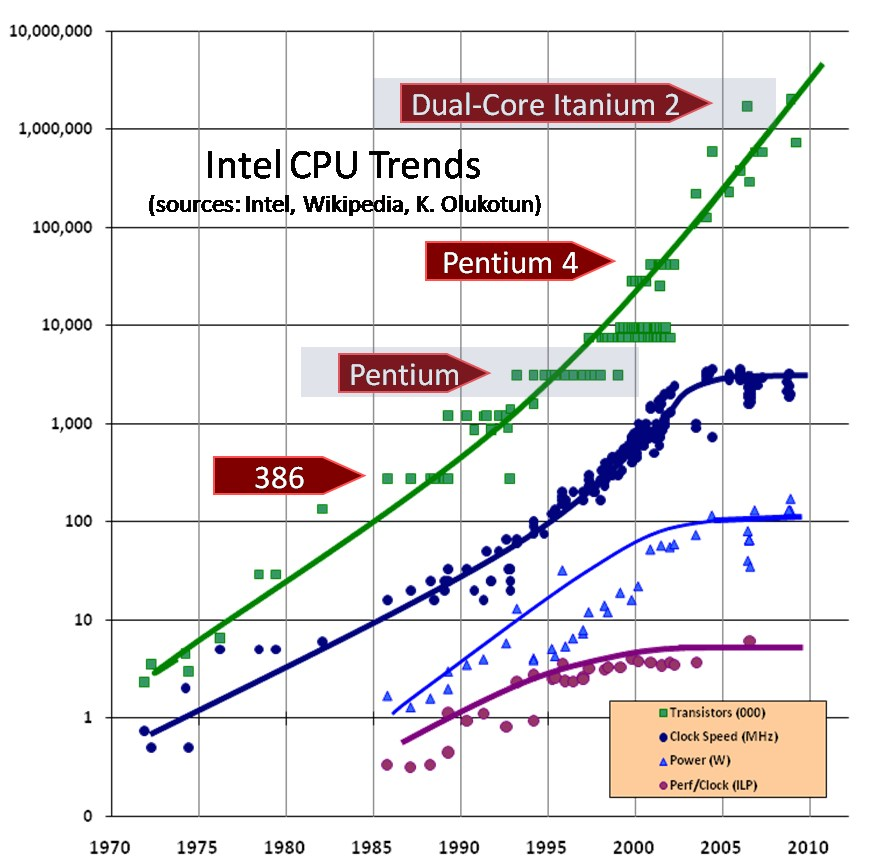
\includegraphics[width=\textwidth]{chap1/Figures/CPU-Scaling.jpg}
	\caption{Intel处理器的发展趋势}
	\label{fig:intelProcessor}
\end{figure}
但是当单个处理器的制造工艺到达纳米级别后,受制于量子效应已经无法进一步提高单个处理器的时钟频率。
随后业界开始转而使用多核系统(Multi-core system),直至目前出现的众核系统(Manycore system)来提升超算的性能。目前最权威的HPC超算
集群排行榜Top500给出的结果显示,无论是排名第一的机器还是所有500强计算能力的综合都较好地符合摩尔定律逐年增长。
\begin{figure}
	\centering
	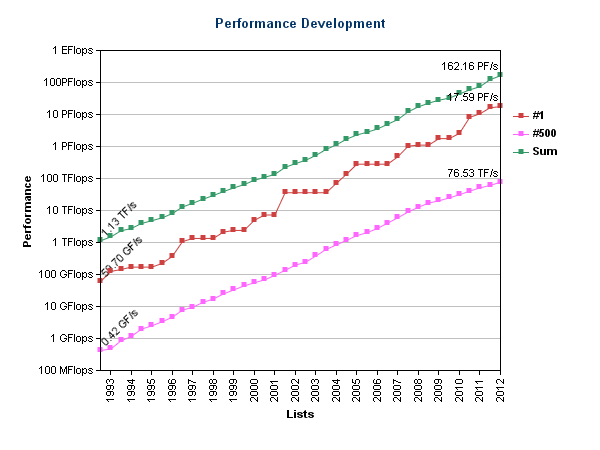
\includegraphics[width=\textwidth]{chap1/Figures/top500Perf.png}
	\caption{Top500超算集群的性能发展}
	\label{fig:top500Perf}
\end{figure}
但是这些峰值运算速度仅仅代表了理论上一台超算集群能够达到的速度,其测试结果也是通过相对简单地基准程序(benchmark)获得的,而真正复杂的应用程序大多数
还未能在超算集群上跑出好的使用效率。目前的应用


% section 高兴能计算的产生和发展 (end)

\section{金融领域的超算应用} % (fold)
\label{sec:intro-finance}

% section 金融领域的超算应用 (end)




% presente our subject and the modeling  
\chapter{课题陈述}
\label{chp:2}

本文所要研究的金融问题是基于欧洲式期权的离散时间对冲策略的风险控制。欧式期权(European Option) 是期权的一种类型。另外两种期权类型是美式期权
(American Option)和亚洲期权(Asian Option)。期权本质上是一种金融合约,它授予期权的拥有者(买方)一种在某一特定时间点或之前,以某一个在合约中给出的价格
(strike price) 购买或者出售某一种金融产品(underlying asset) 的权利。买家在执行自己的权利时,卖家必须按照合约规定的价格进行交易,
但买家同时需要付给买家一定的额外交易手续费(premium)。期权的研究主要集中在对其价值的评估。期权的价值一般可以分为两个部分。一是期权的内部价值
(intrinsic value),主要由该期权基于的金融产品在交易时的市场价格和合约定价的差值决定。二是期权的时间价值(Time Value),这一部分取决于交易前的其他因素如
利息,增值等。期权的研究从19世纪就开始了,但目前的研究一般都是基于1973年提出的Black-Scholes模型。我们的课题也是基于Black-Scholes模型,并对欧式期权
对冲策略的风险控制进行研究。

\section{欧式期权} % (fold)
\label{sec:euroOption}

欧式期权的特点在于买方必须在合约规定的时间到期时才能行使权力。通常将欧式期权的合理价格价定为其期望价值。
相比与美式期权,二者在执行时间上有所不同。
美式期权合同在到期日前的任何时候或在到期日都可以执行合同,结算日则是在履约日之后的一天或两天,
大多数的美式期权合同允许持有者在交易日到履约日之间随时履约,但也有一些合同规定一段比较短的时间可以履约,如“到期日前两周”。
欧式期权合同要求其持有者只能在到期日履行合同,结算日是履约后的一天或两天。目前国内的外汇期权交易都是采用的欧式期权合同方式。
通过比较,结论是:欧式期权本少利大,但在获利的时间上不具灵活性;美式期权虽然灵活,但付费十分昂贵。因此,国际上大部分的期权交易都是欧式期权。
中国国内银行设立的外汇期权业务都是采用的欧式期权交易。

% section 欧式期权 (end)

\section{Black-Scholes模型} % (fold)
\label{sec:BlackScholes}

Black-Scholes 是一个70年代由Fischer Black和Myron Scholes 提出的用于金融衍生品交易的数学模型。这个模型可以推出Black-Scholes公式,
并用于预测欧式期权定价的理论值。70年代至今在众多的实际交易中,该公式的预测估值被认为是非常接近实际观测到的价值。
这个模型的成功也直接导致了期权交易市场的繁荣,并能使芝加哥期权交易市场等大的期权交易场所得到科学的有效的监管。
Black-Scholes 公式是一个偏微分方程,用于预测期权价格随时间的变化。而该模型背后的策略则是通过合理地买卖期权来对冲风险,这种对冲策略被
成为"Delta Hedging",这也是许多更复杂的对冲机构策略的基础。此后Robert C. Merton 进一步发展了该模型,并和Schole分享了1997年的诺贝尔经济学奖。


% section Black-Scholes模型 (end)

\section{课题表述} % (fold)
\label{sec:subject}

本课题研究的对象就是欧式期权利用对冲策略来降低交易的风险。
我们考虑基于Black-Scholes模型的Delta 对冲策略,该策略为一个连续时间策略,也即策略所要求的交易行为发生在每时每刻,关于时间轴连续。
我们知道现实生活中,交易只能发生在一些离散的时间点上, 即交易员只能在一系列相继的时刻点上交易。
一个总所周知的事实是,实际中想要完美的复制实现一个给定的连续时间策略是不可能的。
本课题研究的就是离散时间版本的Delta 对冲策略与理论上的Delta 对冲策略之间的误差及风险控制。
文章\cite{WhenIsTimeContinuous,DiscreteTimeHedgingErrors,Hayashi05evaluatinghedging} 研究了连续时间和离散时间金融交易模型的关系,
但这些文章更多的关注了两者的渐进性质而没有考虑如何最优的复制连续时间策略。本文将弥补这一空白。

在一般化的 Black-Scholes 模型中, 假设在时刻$t$, 期权所基于的风险资产价格为 $X_t$, 另外有一无风险资产价格为 $S_t^0$。
$X_t$ 满足如下的一维随机偏微分方程:
\begin{equation}
dX_t=\mu(X_t)X_tdt+\sigma(X_t)X_tdB_t,
\end{equation}
$X_0=x_0>0, \sigma(x)>0, \forall x>0$,
而无风险资产价格满足一个常微分方程:
\begin{equation}
dS_t^0=rS^0_tdt
\end{equation}。
我们引进一个新的随机过程$W_t$:
\begin{equation}
W_t=B_t+\int^t_0\frac{\mu(X_s)-r}{\sigma(X_s)}ds
\end{equation},
在中性风险的概率空间下,这个随机过程是一个标准的布朗运动。 我们在此中性风险概率空间下考虑问题。
现在风险资产所满足的随机微分方程变为如下形式:
\begin{equation}
dX_t=rX_tdt+\sigma(X_t)X_tdW_t
\end{equation}
我们假设考虑的问题满足如下两个条件:

$(\mathcal{H}_1)$ $\mu$ 和 $\sigma$ 有限的, 两次连续可微且二次偏微分满足 Holder 条件. 更准确的来说, 令 $\hat{\mu}(x)=\mu(exp(x))$, $\hat{\sigma}(x)=\sigma(exp(x))$, 且 $\delta\in (0,1)$, $K>0$, 对任意 $(x,x')\in \mathbb{R}^2$, 我们有:
\begin{equation}
|\hat{\mu}'(x)|+|\hat{\mu}''(x)|+\frac{|\hat{\mu}''(x)-\hat{\mu}''(x')|}{|x-x'|^\delta}+|\hat{\sigma}'(x)|+|\hat{\sigma}''(x)|+\frac{|\hat{\sigma}''(x)-\hat{\sigma''}(x')|}{|x-x'|^\delta}<K.
\end{equation}

$(\mathcal{H}_2)$ 存在$\sigma_0>0$ 使得对任意 $x>0$ 有$|\sigma(x)|\geq \sigma_0$。

在这两个条件下
若欧洲期权的回报函数为 $f\in L^2(X_t)$, 则该期权在$0$ 时刻的价格由下面公式给出:
\begin{equation}
h(f)(x_0)=\mathbb{E}(exp(-rT)f(X_T)|X_0=x_0).
\end{equation}
令
\begin{equation}
u(t, x)=\mathbb{E}(e^{-r(T-t)}f(X_{T-t}^x)),
\end{equation}
则$u$ 是如下方程的解:
\begin{equation}
-\frac{\partial}{\partial t}u(t, x) =\frac{1}{2}\sigma^2(x)x^2\frac{\partial^2}{\partial x^2}u(t,x)+rx\frac{\partial}{\partial x}u(t,x)-ru(t,x)
\end{equation}
这里 $(t,x)\in [0,T)\times (0,\infty)$ 且 $u(0,x)=h(f)$,  $u(T,x)=f(x)$。

一个广为人知的期权定价公式如下:
\begin{equation}
e^{-rT}f(X_T)=h(f)+\int_0^T \xi_t d\widetilde{X}_t
\end{equation}
这里 $\widetilde{X}_t=e^{-rT}X_t$ 是风险资产的折旧贴现价格。 
Ito's 公式给出了Delta 对冲策略$\xi$: 
\begin{equation}
\xi_t=\frac{\partial u}{\partial x}(t, X_t)
\end{equation}
换句话说,为了达到完美对冲,交易员需要在 
$t\in [0, T]$ 的时间内无时不刻的交易, 并且使自己在时刻 $t$ 持有恰好 $\xi_t$ 单位的风险资产。 
这在现实中是不可能达到的。

一个替代的解决方案是用在离散的时刻点交易的方法来逼近原先的对冲策略。假设交易员在$t\in[0, T)$
时间内交易$N$ 次,交易时间被定义为$t_k=kT/N$, $(k\in \{0,...,N\})$, 在 $t\in [t_k, t_{k+1})$时间内,
交易员使自己持有$\xi_{t_k}$单位的风险资产$X_t$。在此离散化策略的逼近下,在期权到期时刻$T$, 
完美对冲和离散化对冲的差值为:
\begin{equation}
\begin{split}
M_T^N
&=e^{-rT}f(X_T)-(u(0,x)+\int_0^T\frac{\partial u}{\partial x}(\varphi(t), 
X_{\varphi_t}))d\widetilde{X}_t\\
&=\int_0^T\frac{\partial u}{\partial x}(t, X_t)d\widetilde{X}_t-\int_0^T\frac{\partial u}{\partial x}(\varphi(t), X_{\varphi(t)})d\widetilde{X}_t\\
&=(X_T-K)^+-\mathbb{E}[(X_T-K)^+]-\int_0^T\frac{\partial u}{\partial x}(\varphi(t), X_{\varphi(t)})dX_t\\
&=(X_T-K)^+-x_0N(d_1(0))+KN(d_2(0))-\sum_{i=0}^{n-1}N(d_1(t_i))(X_{t_{i+1}}-X_{t_i})\\
&=(X_T-K)^+-\frac{x_0}{\sqrt{2\pi}}\int_{-\infty}^{\frac{\log(\frac{x_0}{K})+\frac{1}{2}\sigma^2T}
{\sigma\sqrt{T}}}e^{-\frac{v^2}{2}}dv+\frac{K}{\sqrt{2\pi}}\int_{-\infty}^{\frac{\log(\frac{x_0}{K})-\frac{1}{2}\sigma^2T}{\sigma\sqrt{T}}}e^{-\frac{v^2}{2}}dv\\
&-\sum_{i=0}^{n-1}\frac{1}{\sqrt{2\pi}}\int_{-\infty}^{\frac{\log(\frac{X_{t_i}}{K})+\frac{1}{2}\sigma^2(T-t_i)}{\sigma\sqrt{T-t_i}}}e^{-\frac{v^2}{2}}dv(X_{t_{i+1}}-X_{t_i})\\
\end{split}
\end{equation}
这里 $\varphi(t)=sup\{t_i | t_i\leq t \}$.

对于该误差$M_T^N$,我们已知它有如下的渐进性质:
%\begin{Theorem}
$M_T^N$ 在概率上趋向于0:
\begin{equation}
M_T^N\xlongrightarrow[N\rightarrow +\infty]{\mathbb{P}}0
\end{equation}
%\end{Theorem}
证明:见\cite{ContinuousMartingaleAndBrownianMotion}
%\begin{Theorem}

令 $X_t$ 随机偏微分方程 $dX_t=\sigma(X_t)X_tdW_t$ 的解所对应的随机过程, $u$ 如前文定义, 则我们有 
\begin{equation}
\sqrt{n}M_T^N\xlongrightarrow[N\rightarrow +\infty]{d} \hat{W}_\tau
\end{equation}
这里 $\tau=\frac{1}{2}\int_0^T(\frac{\partial^2 u}{\partial x^2}(t,X_t))^2\sigma^4(X_t)X_t^4dt$, 且 $\hat{W}$ 是一个独立于 $\tau$另一个布朗运动.
%\end{Theorem}
证明:见\cite{rootzen1980}

上面的两条渐进性质不仅告诉我们随着 $N$的增大,离散对冲策略的逼近将越来越成功,两者相差的误差将在概率意义下趋于零,而且还告诉我们此误差的渐进表现
类似于一个系数逐渐变小的布朗运动。特别的,我们从中可知,通过增大 $N$, 在概率意义下,离散化的Delta 对冲策略可以任意程度的逼近完美Delta 对冲策略。

由于实际交易中交易成本一类的问题,所以在一定的交易风险范围内,我们希望能够用最少的交易次数来完成既定的交易策略。
也即我们希望找到一个最小的交易次数$N$来最优化交易成本。
假设在$t=T$时,交易的误差可表示为$|P(X) - P_{T_N}(X)|$, 而可接受的最大误差为$\epsilon$,我们将采用蒙特卡洛模拟算法,通过$M$次模拟,计算出
$|P(X) - P_{T_N}(X)| < \epsilon$的概率$Prob(M,N)$, 当$Prob(M,N)$的值大于一个预先设定的概率值时,我们认为$N$是一个可接受的抽样次数。
算法\ref{alg:bserror} 给出了我们计算验证一个$N$值的串行算法伪代码。

\begin{algorithm}
  \caption{欧式期权对冲策略误差控制的串行算法}
  \label{alg:bserror}
	\begin{algorithmic}[1]
	 \Require $X_0$ \Comment{金融产品在$t=0$时的初始价格}
	 \Require $\sigma$ \Comment{市场波动性}
	 \Require $K$ \Comment{期权合约价格}
	 \Require $T$ \Comment{期权到期时间}
	 \Require $\epsilon$ \Comment{可接受的误差上限}
         \Require $N_{0}$ \Comment{理论给出的初始离散抽样次数上界}
         \Require $M$ \Comment{蒙特卡洛模拟次数}
         \Ensure $prob$
	 \Procedure{BSERROR}{M, N}
         \State $error \gets 0$ \Comment{离散策略和连续策略的误差}
         \State $NRV[N]$ \Comment{符合正态分布的N个独立随机数}
         \State $BM[N]$ \Comment{布朗运动的N个状态}
         \State $PX[N+1]$ \Comment{在离散时间点的期权价格}
	 \State $\delta t \gets T/N$ \Comment{时间间隔}
	 \State $count \gets 0$ \Comment{在$M$次模拟中$N$被接受的次数}
         \State $N \gets N_0$
	  \For{$m=1:M$} \Comment{M次蒙特卡洛模拟}
          \State $error \gets 0$ \Comment{离散策略和连续策略的误差}
	  \ForAll {$NRV[j]$}
	     $NRV[j] \gets GaussianNumGenerator()$
	  \EndFor
	  \State $BM[0] \gets NRV[0] \cdot \sqrt{\delta t}$ 
	  \ForAll {$BM[j]$}
	     $BM[j] \gets BM[j-1] + NRV[j]\cdot \sqrt{\delta t}$ 
	  \EndFor
	  \State $PX[0] \gets X0$
	  \ForAll {$j= 1:N+1$}
	  \State $PX[j]\gets X0 \cdot exp(-0.5\cdot \sigma^2 \cdot j \cdot \delta t + \sigma \cdot BM[j-1])$
	  \EndFor
	  \ForAll{$j=0:N-1$}
	  \State $Upper \gets (\log(PX[j]/K) + 0.5\cdot \sigma^2 \cdot (T- T_j))/ (\sigma \cdot \sqrt{T-T_j})$ 
	  \State $error \gets error - 1/(\sqrt{2\pi}) \cdot (PX[j+1]-PX[j])\cdot \int_{-\infty}^{Upper}e^{-t^2/2}dt $
	  \EndFor

	  \If {$PX[N] > K$} 
	  \State $error \gets error + (PX[N]-K)$
	  \EndIf

	  \State $Upper1 \gets (log(X0/K) + 0.5\cdot \sigma^2 \cdot T)/(\sigma \sqrt{T})$
	  \State $Upper2 \gets (log(X0/K) - 0.5\cdot \sigma^2 \cdot T)/(\sigma \sqrt{T})$
	  \State $error = error + K/\sqrt{2\pi} \cdot \int_{-\infty}^{Upper2}e^{-t^2/2}dt -X0/\sqrt{2\pi}\cdot \int_{-\infty}^{Upper1}e^{-t^2/2}dt$
	  
	  \If {$error < \epsilon$} 
	  \State $count \gets count + 1$ 
	  \EndIf
	  \EndFor

	  \State $prob \gets count/M$
	  \State return $prob$
	 \EndProcedure
  \end{algorithmic}
\end{algorithm}


% section 课题表述 (end)

%\section{BSERROR算法的并行化} % (fold)
%\label{sec:BSERRORParallel}



% section BSERROR算法的并行化 (end)


% algorithm for choosing initial N and M
\chapter{参数选择及收敛条件}
\label{chp:3}
我们进行 M 次模特卡罗模拟实验,对于每一次模拟,选取某个 $N$, 计算相应的误差$M_T^N$, 我们希望该误差小于可接受的最大误差 $\epsilon=X0*10^{-3}$。 
我们用蒙特卡洛的方法计算 $M_T^N\leq \epsilon$ 的概率,并希望该概率能超过某一个特定值: $Prob=95\%$。 
在这个问题中 $M$ 和 $N$ 的初始值以及其更新方法至关重要。 对$M$ 而言, 一方面较大的 $M$ 会增大模特卡罗方法以及通过此方法计算出来的概率的可信度,另一方面
$M$ 过大,将不可避免的造成更高的资源和硬件的要求,如何在保持一定可行度的条件下选择一个较小的 $M$ 需要一个精巧的方法。
对 $N$ 而言,较大的 $N$ 会使得逼近更准确,从而误差 $M_T^N$ 较小,但也会造成资源的浪费和迭代收敛的过程冗长。
较大或者较小的 $M$ 和 $N$ 的初始值将导致收敛缓慢甚至不收敛。
如何选择合适的 $M$ 和 $N$ 的初始值,
如何让它们互相迭代更新, 以及怎样判断收敛与否是本章所需要解决的问题。
\section{参数 N} % (fold)
\label{sec:N}
关于 $N$ 的初始值的选取,一个首要的问题是,数值模拟中,$M$ 会影响我们对 $N$ 的判断,甚至一个选取不好的 $M$ 会给出错误的 $N$ 的更新方向,从而导致问题
得不到收敛。为了避免这种问题, 我们在这里给出一种不依赖于 $M$ 的 $N$ 的初始值选定方法。

我们需要一个尽可能小的 $N$, 使得存在某个关于 $N$ 的函数 $P(N)$,如下不等式成立:
\begin{equation}
Probability(M_T^N\geq\epsilon)=\mathbb{P}(M_T^N\geq\epsilon)<P(N)。
\end{equation}
若我们能发现这样的函数$P(N)$,则所有满足不等式:
\begin{equation}
P(N)\leq 1-Prob=5\% 
\end{equation}
的正整数 $N$, 都满足 $\mathbb{P}(M_T^N<\epsilon)>Prob=95\%$。
我们只需要取满足不等式的最小的正整数 $N$ 即可。此时 $N$ 的选取独立于 $M$, 也即无论我们选取怎样的$M$, 理论上都会有 $\mathbb{P}(M_T^N<\epsilon)>Prob$ 成立。

为了寻找函数 $P(N)$, 我们先引入两个引理,

\textbf{(Burkholder-Davis-Gundy inequality)}
令 $T>0$,$(M_t)_{0\leq t\leq T}$ 为一个局部的鞅,且 $M_0=0$. 则对于所有的 $0<p<+\infty$, 存在独立于 $T$ 和 $(M_t)_{0\leq t\leq T}$ 的常数
$c_p$,$C_p$, 使得 
\begin{equation}
c_p\mathbb{E}[\left \langle M \right \rangle_T^{\frac{p}{2}}]\leq \mathbb{E}[(sup_{0\leq t\leq T}|M_t|)^p]\leq C_p\mathbb{E}[\left \langle M \right \rangle_T^{\frac{p}{2}}]
\end{equation}
See XXXXXX.

In paper XXXXXX, 作者证明了 $C_p\leq (2\sqrt{p})^p$.

\textbf{(Generalized Minkowski inequality)}
设 $(S_1,\mu_1)$ 和 $(S_2,\mu_2)$ 是两个可测空间,且 $F : S_1\times S_2\rightarrow R$ 为可测映射. 
则广义的Minkowski 积分不等式是:
\begin{equation}
(\int_{S_2}|\int_{S_1}F(x,y)d\mu_1(x)|^pd\mu_2(y))^{\frac{1}{p}}\leq \int_{S_1}(\int_{S_2}|F(x,y)|^pd\mu_2(y))^{\frac{1}{p}}d\mu_1(x), \forall p\geq 1
\end{equation}
See XXXXXX for a proof

不失一般性, 在以下的计算中我们设 $r=0$, $\sigma(X_t)=constant=\sigma>0$ 回报函数 $f(x)=(x-K)^{+}, K>0$.  

由 Chebyshev 不等式, 我们有 
$$\mathbb{P}(M_T^n\geq \gamma)\leq \frac{E[(M_T^n)^p]}{\gamma^p}, \forall p>0$$

再由 Burkholder-Davis-Gundy 不等式有: 
\[
\mathbb{E}[(M_T^n)^p]\leq C(p)\mathbb{E}[\left \langle M^n \right \rangle_T^{\frac{p}{2}}]
\]
这里我们用已知最优的结果 $C(p)=(2\sqrt{p})^p$.

对方程XXXXXXX, 关于 $x$ 微分,我们有
\begin{equation}
\frac{\partial^2 u}{\partial t \partial x}(t, x) +\frac{1}{2}\sigma^2x^2\frac{\partial^3}{\partial x^3}u(t,x)=
-\sigma^2x\frac{\partial^2u}{\partial x^2}(t, x)
\end{equation}
对$\frac{\partial u}{\partial x}(t, X_t)-\frac{\partial u}{\partial x}(\varphi(t), X_{\varphi(t)})$ ,从 $\varphi(t)$ 到 $t$ 使用 It$\hat{o}$ 公式。
结合方程 XXXXXX, 我们有
\[
\begin{split}
&\frac{\partial u}{\partial x}(t, X_t)-\frac{\partial u}{\partial x}(\varphi(t), X_{\varphi(t)})\\
&=\int_{\varphi(t)}^t (\frac{\partial^2 u}{\partial x\partial t}(\theta, 
X_\theta)+\frac{1}{2}\frac{\partial^3 u}{\partial x^3}(\theta, X_\theta)\sigma^2X^2_\theta) d\theta
+ \int_{\varphi(t)}^t \frac{\partial^2 u}{\partial x^2}(\theta, X_\theta)\sigma X_\theta dW_\theta\\
&=  \int_{\varphi(t)}^t \frac{\partial^2 u}{\partial x^2}(\theta, X_\theta)\sigma X_\theta (dW_\theta-\sigma d\theta)\\
\end{split}
\]

所以
\[
M_T^n=\int_0^T\int_{\varphi(t)}^t \frac{\partial^2 u}{\partial x^2}(\theta, X_\theta)\sigma X_\theta (dW_\theta-\sigma d\theta)\sigma X_t dW_t
\]
\[
\left \langle M^n \right \rangle_T=\int_0^T(\int_{\varphi(t)}^t \frac{\partial^2 u}{\partial x^2}(\theta, X_\theta)\sigma X_\theta (dW_\theta-\sigma d\theta))^2\sigma^2 X_t^2 dt
\]

我们假设 $p\geq 2$. 由广义 Minkowshi 不等式, 我们有:
\[
\begin{split} 
\mathbb{E}[\left \langle M^n \right \rangle_T^{\frac{p}{2}}]
&=\mathbb{E}[(\int_0^T(\int_{\varphi(t)}^t \frac{\partial^2 u}{\partial x^2}(\theta, X_\theta)\sigma X_\theta (dW_\theta-\sigma d\theta))^2\sigma^2 X_t^2 dt)^{\frac{p}{2}}]\\
&\leq (\int_0^T(\mathbb{E}[(\int_{\varphi(t)}^t \frac{\partial^2 u}{\partial x^2}(\theta, X_\theta)\sigma X_\theta (dW_\theta-\sigma d\theta))^p\sigma^p X_t^p] )^{\frac{2}{p}}dt)^{\frac{p}{2}}\\
\end{split}
\]
考虑一个满足下面条件的新的概率$\widetilde{\mathbb{Q}}$: 
$$\frac{d\widetilde{\mathbb{Q}}}{d\mathbb{Q}}=e^{\sigma W_t-\frac{\sigma^2t}{2}}=\frac{X_t}{X_0}$$ 
则在此新的概率$\widetilde{\mathbb{Q}}$ 下,$\widetilde{W}_t=W_t-\sigma t$ 是一个布朗运动。

由Cauchy 不等式,在概率 $\widetilde{\mathbb{Q}}$ 下, 我们有:
\[
\mathbb{E}[\left \langle M^n \right \rangle_T^{\frac{p}{2}}]\leq x_0
(\int_0^T(\mathbb{E}_{\widetilde{\mathbb{Q}}}[(\int_{\varphi(t)}^t \frac{\partial^2 u}{\partial x^2}(\theta, X_\theta)\sigma X_\theta d\widetilde{W}_\theta)^{2p}])^{\frac{1}{p}}(\mathbb{E}[\sigma^{2p} X_t^{2p-2}] )^{\frac{1}{p}}dt)^{\frac{p}{2}}
\]
再次使用Burkholder-Davis-Gundy 不等式和广义 Minkowski 不等式,我们有:
\[
\begin{split}
\mathbb{E}[\left \langle M^n \right \rangle_T^{\frac{p}{2}}]&\leq x_0
(\int_0^T(C(2p)\mathbb{E}_{\widetilde{\mathbb{Q}}}[(\int_{\varphi(t)}^t (\frac{\partial^2 u}{\partial x^2}(\theta, X_\theta)\sigma X_\theta)^2 d\theta)^{p}])^{\frac{1}{p}}(\mathbb{E}[\sigma^{2p} X_t^{2p-2}] )^{\frac{1}{p}}dt)^{\frac{p}{2}}\\
&\leq x_0C(2p)^{\frac{1}{2}}(\int_0^T(\int_{\varphi(t)}^t(\mathbb{E}_{\widetilde{\mathbb{Q}}}[ (\frac{\partial^2 u}{\partial x^2}(\theta, X_\theta)\sigma X_\theta)^{2p}])^{\frac{1}{p}} d\theta)(\mathbb{E}[\sigma^{2p} X_t^{2p-2}] )^{\frac{1}{p}}dt)^{\frac{p}{2}}\\
\end{split}
\]
\[
\begin{split}
\mathbb{E}[X_t^{2p-2}]&=X_0^{2p-2}\mathbb{E}[e^{(2\sigma W_t-\sigma^2t)(p-1)}]\\
&=X_0^{2p-2}e^{2t(p-1)^2\sigma^2-p(t-1)\sigma^2}\\
&\leq
X_0^{2p-2}e^{\sigma^2p}, \forall p\in [2, +\infty)\\
\end{split}
\]
定义$\widetilde{C}(p)$ 如下 
\[
\widetilde{C}(p)=
X_0^{2p-2}e^{\sigma^2p}, \forall p\in  [2, +\infty)
\]
另一方面我们有:
\[
\mathbb{E}_{\widetilde{\mathbb{Q}}}[ (\frac{\partial^2 u}{\partial x^2}(\theta, X_\theta)\sigma X_\theta)^{2p}]=\frac{1}{(T-\theta)^p}\mathbb{E}_{\widetilde{\mathbb{Q}}}[N(d_1(\theta))^{2p}]
\]
这里
\[
N(x)=\frac{1}{\sqrt{2\pi}}e^{\frac{-x^2}{2}}, d_1(\theta)=\frac{1}{\sigma\sqrt{T-\theta}}(log(\frac{X_\theta}{K})+\frac{1}{2}(T-\theta))
\]
记 $d_2(\theta)=\frac{1}{\sigma\sqrt{T-\theta}}(log(\frac{X_\theta}{K})-\frac{1}{2}(T-\theta))$, 此定义将在后面用到.
\textbf{注} 
For more details, see \cite{mathematique}

由$X_t=x_0exp(\sigma \widetilde{W}_t+\frac{1}{2}\sigma^2t)$, 我们有:
\[
\mathbb{E}_{\widetilde{\mathbb{Q}}}[ (\frac{\partial^2 u}{\partial x^2}(\theta, X_\theta)\sigma X_\theta)^{2p}]
=(\frac{1}{2\pi(T-\theta)})^p\mathbb{E}_{\widetilde{\mathbb{Q}}}[exp(-p(\frac{log(\frac{x_0}{K})+\frac{1}{2}\sigma^2T+\sigma\widetilde{W}_{\theta}}{\sigma\sqrt{T-\theta}})^2)]
\]
定义常数$\lambda$ 如下: $\lambda=log(\frac{x_0}{K})+\frac{1}{2}\sigma^2T$, 则不等式为:
\[
\begin{split}
\mathbb{E}_{\widetilde{\mathbb{Q}}}[ (\frac{\partial^2 u}{\partial x^2}(\theta, X_\theta)\sigma X_\theta)^{2p}]
&=(\frac{1}{2\pi(T-\theta)})^p\int^{+\infty}_{-\infty}\frac{1}{\sqrt{2\pi\theta}}e^{-\frac{z^2}{2\theta}}e^{-\frac{p}{T-\theta}(z+\frac{\lambda}{\sigma})^2}dz\\
&=(\frac{1}{2\pi(T-\theta)})^p\sqrt{\frac{T-\theta}{T-\theta+2p\theta}}e^{-\frac{p}{T-\theta+2p\theta}\frac{\lambda^2}{\sigma^2}}\\
&\leq \frac{\sqrt{T-\theta}}{(2\pi(T-\theta))^p}\frac{\sigma}{\lambda\sqrt{2p}}e^{-\frac{1}{2}}\\
\end{split}
\]
所以 
\[
\begin{split}
\mathbb{E}[\left \langle M^n \right \rangle_T^{\frac{p}{2}}]&\leq
 x_0C(2p)^{\frac{1}{2}}(\int_0^T(\int_{\varphi(t)}^t (T-\theta)^{\frac{1}{2p}-1} d\theta)\frac{1}{2\pi}(\frac{\sigma}{\sqrt{2p}\lambda}e^{-\frac{1}{2}})^{\frac{1}{p}}x_0^{2-\frac{2}{p}}e^{\sigma^2}dt)^{\frac{p}{2}}\\
 &=x_0^pC(2p)^{\frac{1}{2}}(\frac{1}{2\pi})^{\frac{p}{2}}(\frac{\sigma}{\lambda\sqrt{2\pi}})^{\frac{1}{2}}e^{\frac{2\sigma^2p-1}{4}}
 (\int_0^T\int_{\varphi(t)}^t (T-\theta)^{\frac{1}{2p}-1} d\theta dt)^{\frac{p}{2}}\\
 \end{split}
 \]
 \[
 \begin{split}
 (\int_0^T\int_{\varphi(t)}^t (T-\theta)^{\frac{1}{2p}-1} d\theta dt)^{\frac{p}{2}}
 &=(2p\int_0^T((T-\varphi(t))^{\frac{1}{2p}}-(T-t)^{\frac{1}{2p}}) dt)^{\frac{p}{2}}\\
 &=(2p\frac{T}{n}\sum_{i=0}^{n-1}(T-t_i)^{\frac{1}{2p}}-\int_0^T(T-t)^{\frac{1}{2p}} dt)^{\frac{p}{2}}\\
 &=(2p)^{\frac{p}{2}}(\frac{T}{n})^{\frac{2p+1}{4}}(\sum_{i=1}^{n}i^{\frac{1}{2p}}-\int_0^n(n-v)^{\frac{1}{2p}} dv)^{\frac{p}{2}}\\
 &=(2p)^{\frac{p}{2}}(\frac{T}{n})^{\frac{2p+1}{4}}(\sum_{i=1}^{n}i^{\frac{1}{2p}}-\frac{2p}{2p+1}n^{\frac{2p+1}{2p}})^{\frac{p}{2}}\\
 \end{split}
 \]
 由于$0<\frac{1}{2p}=q<1$, 我们知道函数 $g(x)=x^q$ 是凹函数(concave). 由$g(x)$的凹性质,我们有:
 \[
 \sum_{i=1}^{n-1}i^q+\sum_{i=1}^{n-1}\frac{(i+1)^q-i^q}{2}<\int_1^{n}x^qdx
 \]
 所以
 \[
 \begin{split}
 \sum_{i=1}^{n-1}i^q
 &<\frac{1}{q+1}(n^{q+1}-1)-\frac{1}{2}(n^q-1)\\
 &<\frac{n^{q+1}}{q+1}-\frac{n^q}{2}\\
 \end{split}
 \]
 \[
 \sum_{i=1}^{n}i^q=\sum_{i=1}^{n-1}i^q+n^q<\frac{n^{q+1}}{q+1}+\frac{n^q}{2}
 \]

 \[
 \sum_{i=1}^{n}i^{\frac{1}{2p}}-\frac{2p}{2p+1}n^{\frac{2p+1}{2p}}<\frac{n^{\frac{1}{2p}}}{2}
 \]
 因此:
 \[
 \begin{split}
 \mathbb{E}[\left \langle M^n \right \rangle_T^{\frac{p}{2}}]
 &\leq x_0^pC(2p)^{\frac{1}{2}}(\frac{1}{2\pi})^{\frac{p}{2}}(\frac{\sigma}{\lambda\sqrt{2\pi}})^{\frac{1}{2}}e^{\frac{2\sigma^2p-1}{4}}
 (2p)^{\frac{p}{2}}(\frac{T}{n})^{\frac{2p+1}{4}}(\frac{1}{2})^{\frac{p}{2}}n^{\frac{1}{4}}\\
 \end{split}
 \]
 故而对于 $p\geq 2$,
 \[
 \mathbb{P}(M_T^n\geq \gamma)\leq L(p)=C_0\frac{1}{\gamma^p}C(p)x_0^pC(2p)^{\frac{1}{2}}(\frac{1}{2\pi})^{\frac{p}{2}}e^{\frac{\sigma^2p}{2}}
 p^{\frac{p}{2}}(\frac{T}{n})^{\frac{p}{2}}
 \]
 这里
 $C_0=T^{\frac{1}{4}}(\frac{\sigma}{\lambda\sqrt{2\pi}})^{\frac{1}{2}}e^{-\frac{1}{4}}$ 是一个与$p, n$ 无关的常数。  
 通过令等式 $\frac{\partial \log(L(p))}{\partial p}=0$ 成立。 我们找到最优的 $p$。
 \[
 \log(L(p))=\frac{3}{2}p\log(p)+\log(C_0)-\frac{p}{2}\log(C_1n)
 \]
 这里 $C_1=\frac{\gamma^2\pi e^{-\sigma^2}}{16x_0^2T}$ 是与 $p, n$ 无关的常数。
 \[
 0=\frac{\partial\log(L(p))}{\partial p}=\frac{1}{2}(3+3\log(p)-\log(C_1n)) 
 \]
 \[
 p=\frac{(C_1n)^{\frac{1}{3}}}{e}
 \]
 最优的$p$ 是 $p*$:
 \[
 p*=
 \begin{cases}
 2, \quad  \log(C_1n)<3\log(2)+3\\
 \frac{(C_1n)^{\frac{1}{3}}}{e}, \quad \log(C_1n)\geq 3\log(2)+3\\
 \end{cases}
 \]
 因此 $L(p)$ 的最小值是:
 \[
 L(p*)=
 \begin{cases}
 \frac{8C_0}{C_1n}, \quad \log(C_1n)<3\log(2)+3\\
 C_0e^{-\frac{3(C_1n)^{\frac{1}{3}}}{2e}}, \quad \log(C_1n)\geq 3\log(2)+3\\
 \end{cases}
 \]
 现在我们得到了一个 $N$ 的估界:
 \textbf{Proposition}
 \[
 \mathbb{P}(M_T^n\geq \gamma)\leq 
 \begin{cases}
 \frac{128\sigma^{\frac{1}{2}}x_0^2T^{\frac{5}{4}}e^{\sigma^2}}{e^{\frac{1}{4}}\gamma^2\pi (\log(\frac{x_0}{K})+\frac{1}{2}\sigma^2T)^{\frac{1}{2}}(2\pi)^{\frac{1}{4}}}\frac{1}{n}, \quad \log(C_1n)<3\log(2)+3\\
 T^{\frac{1}{4}}(\frac{\sigma}{(\log(\frac{x_0}{K})+\frac{1}{2}\sigma^2T)\sqrt{2\pi}})^{\frac{1}{2}}e^{-\frac{1}{4}}e^{-\frac{3\gamma^{\frac{2}{3}}\pi^{\frac{1}{3}}}{2ex_0^{\frac{2}{3}}T^{\frac{1}{3}}16^{\frac{1}{3}}e^{\frac{\sigma^2}{3}}}n^{\frac{1}{3}}}, \quad \log(C_1n)\geq 3\log(2)+3\\
 \end{cases}
 \]


% section 参数N (end)

\section{参数M} % (fold)
\label{sec:M}
在确定了 $N$ 的迭代初始值之后 $N_0$,我们可以使用该值来确定一个合适大小的 $M$ 的迭代初始值。
一个合适的 $M$ 的初始值应该满足如下条件:在 $N$ 为其初始迭代值时, $M$ 的值应该使得模特卡罗模拟出的概率 $\mathbb{P}(M_T^N<\epsilon)$ 收敛稳定。
也即,固定$N$ 为其初始值不变,当 $M$ 在其迭代初始值附近扰动时,相应的 $\mathbb{P}(M_T^N<\epsilon)$ 也只是微小扰动。动态调优的技术可以被应用在这里。

在我们的问题背景下,通过动态调优和经验发现,一个较为恰当的 $M$ 初始值可以为 $M=10^6$, 我们通过比较 $M=10^6+i*100$, $i=0,...,10$ 
所对应的 $\mathbb{P}(M_T^N<\epsilon)$来调整 $M$, 若对应的概率在 $10^{-3}$范围内,则将$M$ 减小为原先的一半,否则增大 $M$ 为原先的两倍。
重复此过程,知道发现满足条件的最小的 $M$。 我们然后固定这个最优的 $M$, 然后尝试找出最优的 $N$。

根据前面的理论,最优的 $N$ 存在于 $[0, N_0]$ 区间内。我们仍然使用二分法寻找最优的$N$, 首先我们令 $N_1=N_0/2$, 在此参数下模拟相应的
$\mathbb{P}(M_T^N<\epsilon)$, 若此模拟概率大于 $Prob$, 则令 $N_2=N_1/2$, 反之,则令 $N_2=\frac{N_0+N_1}{2}$。
重复此过程直至找到最优的$N$。

% section 参数M (end)






% parallel scheme
\chapter{并行化算法}
\label{chp:4}

算法并行化的第一步通常是设计一个符合待处理问题及处理器架构特点的并行方案,然后根据该方案确定相应的编程模型,最后分析并行程序的性能,有针对性地做具体的优化。
并行程序的性能优化和普通串行程序有许多共通之处。具体来说主要分为两个大类:针对内存使用的优化和针对for循环的改进。

由于日益增长的处理器速度和发展相对较缓的内存速度之间逐渐拉开了差距,内存通常成为程序蓄能的瓶颈。现代处理器通常采用分层内存体系,高带宽,低延迟(lower latency),低能耗的高速缓存对提升数据局部性(data locality)至关重要。针对缓存优化的方法有很多,例如对齐数据(data alignment)使得缓存的加载更有效率,依据缓存的大小处理相应的数据块(cache blocking),预读取(prefetching)提前将需要处理的数据加载到缓存中,或者通过流式存储技术(streaming store)将非时间相关(nontemporal)的计算结果"绕过"缓存直接写入主内存从而避免"污染"缓存其他数据等。和数据代码缓存一样,页表缓存(Translation Lookaside Buffer)也是影响性能的一个因素。页表缓存存储了一部分标签页表条目,用于改进从虚拟内存地址到物理地址的转译速度,对于特定问题,通过使用不同尺寸的页面大小,重构数据可以避免页表缓存中的热点。

针对for循环优化的一般技术包括循环展开(loop unrolling),分块循环(loop tiling), 循环互换(loop interchange),循环合并(loop fusion),循环偏移(loop skewing),循环剥离(loop peeling)等。这些改进很多时候也是为了更好地使用内存或者为进一步并行化做准备。
目前绝对意义上的串行程序在实际中已不多见,因为在编译过程中编译器会或多或少引入不同程度的并行化处理。然而由于编译器优化的前提是基于代码的正确性,串行程序的逻辑遵循一个绝对的代码执行顺序,因而其编写和调试难度远低于并行程序。并行程序的运行由于同时驱动不同的逻辑运算单元,容易出现数据的竞态条件(race condition)等导致最终结果不确定的因素。本章将着重描述几种针对本课题不同的并行方案,及其具体实现。

\section{并行性分析}
\label{sec:parallelism}
并行的目的就是在充分利用单机资源的基础上,将计算扩展到多个机器,在可接受的时间范围内处理规模更大,复杂度更高的问题。
在单个机器上,原则上我们需要发掘串行算法中的并行机会,将基本的并发性操作表述为任务(task)的形式提交给调度器(scheduler),再由调度器将其分发给不同的线程执行。在MIC这样的众核处理器上,足够的任务级并行度对于充分利用片上丰富的线程资源非常重要。由于时间的限制我们选择不重新实现一个新的调度算法,而是使用现有的工具,如OpenMP,Cilk+或者Threading Building Blocks(TBB)。
在多个节点上,我们采用消息传递模式如MPI来进行通信,目标是尽量降低通信量的同时,将计算和通信重叠起来,提高整体效率。

算法\ref{alg:bserror}描述了欧式期权对冲策略误差控制的串行算法。本章的核心目的就是论述基于该算法的并行化方案。
分析该算法可知蒙特卡洛模拟的结果依赖每次模拟求得的误差$error$,而求$error$的过程除了两项非随机量,其余均与$PX$相关。数组$PX$表示的是在离散时间点的期权价格,取值和一个随机布朗运动的各个状态相关联。该布朗运动可视作一个马尔科夫过程,前后两项相差一个符合高斯分布的随机数。由于其每两项之间存在数据依赖性,使得其并行度十分有限。因此问题的关键在于如何有效地打破这种数据之间的依赖性。本文所讨论的数据依赖性本质上源自于N个独立高斯分布的随机数组成的数组$NRV[N]$。对于一个给定的N和从$BM[N]$中选取的任何一段连续的子集$bm[n]$,如果可以并行地处理这些分段子集,我们就可以极大地提高计算效率,实现本节最初提出的目标。

计算某个子集的条件是已知其初始状态和该子集所对应$NRV[N]$中的子集。而该子集的初始状态可表示为其之前所有状态对应的正态分布随机数之和乘以一个常量。
因此有两种并行思路。第一种是将整个长度为N的数组分为连续的子集,按顺序每次所有的计算资源并发地参与计算其中一段子集,计算完成该段子集之后再计算紧邻的下一段。如此,计算下段子集的时候,它的初态就是上一段的终态加上一个随机数,而上段的终态是已知的。依据这种方案,基本的并行任务(task)是已知某段子集对应的所有的随机数,计算其中某个布朗运动状态,其对应的离散时间点的期权价格,以及最终的误差。

第二种思路是将我们之前所讨论的某段子集的处理直接作为基本的并行任务分配给线程计算。这样的话子集的初始状态是未知的,因为不能假设某个线程先后处理的是连续的子集。在这种情况下,需要根据之前生成的随机数来推断某段子集的初始状态。这就无法回避一个重要的问题,随机数发生器。

在目前的计算机应用里,几乎所有用到的随机数发生器都只能产生伪随机数。其原理通常是根据某种算法计算出一连串在实际应用中可认为相互独立的数。当该算法的结果空间足够大的时候,生成的伪随机数几乎没有可能重复,从而保证了算法的有效性。在该课题中,我们使用的是基于梅森旋转算法(Mersenne twister)的高斯分布随机数发生器,它有$2^{19937}-1$的非常长的周期。该随机数发生器的并行版本,在于生成不同的随机流(stream),不同的流使用不同的“种子(seed)”在不同的结果子空间中计算随机数,相互之间保持独立。

在我们的第一种并行思路中,我们只需要生成一条随机流,每次计算某段子集的时候空闲的线程利用随机数发生器生成下一个紧邻子集对应的随机数。所有随机数由全部线程共享,从而解除了数据的依赖性。
在第二种并行思路中,由于某段子集作为一个基本的任务分配给线程,不同线程间异步地对不同段子集进行操作,因此无法共享单条随机数组。在这种情况下,每个线程保有一条私有的随机数流,根据自己计算的进度按需生成相应的随机数。这种情况下对于数据依赖性的处理则在于随机数的“种子”。对于不同的流使用不同的种子固然是可以得到互相独立的随机数组。但如果使用相同的种子则会生成完全一样的随机数组。由于不同的线程虽然处理的子集不同,但都是针对同一个给定$N$的离散价格误差的计算,$N$个随机数理应一致。通过不同的随机流,不同的线程独立生成随机数,避免了相互之间的通信,从而解除了数据的依赖性。

根据以上提供的两种思路,我们利用Intel OpenMP实现了单机上的并行版本。由于该算法的最终目的是寻找一个最优的$N$以满足给定的可容忍概率。每一次迭代都需要$M$次蒙特卡洛模拟计算一个新的$N$值。在实际中,只有相对较大的$M$值才能得到令人信服的结果。因此对于把单机版本扩展到多个节点或机器,我们选择在$M$这个维度上并行。基本思路是基于Master-Slave模型由一个主机(boss)收集由工作机(worker)发送过来的结果,分析整理之后决定下一次计算的$N$\footnote{关于$N$的最优化搜索具体讨论见第\ref{sec:searchN}节}值并发送给工作机。工作机在等待指令的同时自行选取一个更小的$N$值继续计算。接受到主机指令之后假如自行计算的$N$值和主机指令相同,则继续完成。否则舍弃计算结果重新开始一个新的$N$值的计算。为了更好地重叠计算和通信,我们采用非阻塞通信模式,如此,工作机可以充分发挥计算效能,避免空隙或等待。具体的实现细节参见第\ref{sec:mpi}节。

\section{单机并行算法}
\label{sec:monoparallel}
根据上节\ref{sec:parallelism}的分析,我们分别在算法\label{alg:omp1},\label{alg:omp2_1}和\label{alg:omp2_2}中给出两种单机并行思路的具体实现细节。在实际中,我们采用Intel MKL(Math Kernel Library)提供的高斯分布随机数发生器。该发生器基于梅森旋转算法。每次可生成单个或多个随机数。
\subsection{方案一}
该方案将整段N分为相邻的子集,子集内部连续,所有线程依次对每一段子集进行并行处理。
\begin{algorithm}
  \caption{基于多线程(multithreading)和矢量化(vectorization)的单机并行算法一(单次蒙特卡洛模拟)}
  \label{alg:omp1}
  \begin{algorithmic}[1]
    \Require $X_0, \sigma, K, T, \epsilon, M, N$ (参见算法\ref{alg:bserror})
    \Require $N_{cache}$ \Comment{依序并行处理的子集大小}
    \Ensure $count$
    \Procedure{$MONO_1$}{M, N}
    \State $error \gets 0$
    \State $count \gets 0$
    \State $NRV[N_{cache}] \gets vdRngGaussian(N_{cache})$ \Comment{一次生成$N_{cache}$个符合高斯分布的随机数,赋给线程共享的NRV数组}
    \State $BM[N_{cache}]$ \Comment{线程共享的BM数组}
    \State $PX[N_{cache}+1]$ \Comment{线程共享的PX数组}
    \State $PX[0] \gets 0$
    \State $\delta t \gets T/N$
    \State $BM[0] \gets \sqrt{\delta t} \times NRV[0]$
    \For{$k=1:(int)N/N_{cache}$}
    \State \textbf{Start parallel for region} \Comment{调度器将不同的i分配给不同线程}
    \For{$i=1:N_{cache}$}
    \State $BM[i] = BM[0] + \sqrt{\delta t}\times reduce\_add(NRV[1:i])$ \Comment{闭区间SIMD reduction操作}
    \State $PX[i+1] = X_0 \times \exp(-0.5 \sigma^2 \times (kN_{cache}+i+1) \times \delta t + \sigma \times BM[i])$
    \EndFor
    \State \textbf{End parallel for region}
    \State $PX[1] = X_0 \times \exp(-0.5 \sigma^2 \times (kN_{cache}+1) \times \delta t + \sigma \times BM[0])$
    \State \textbf{Start parallel region reduction(+:error) nowait}
    \For{$i=0:N_{cache}$} 
    \State $j \gets kN_{cache}+1$
    \State $T_j \gets {j \times T}/{N}$
    \State $Upper = (\log(PX[i]/K)+0.5\times \sigma^2 \times (T-T_j))/(\sigma \times \sqrt{T-T_j})$
    \State $error \gets error - \frac{1}{\sqrt{2\pi}}\times (PX[i+1]-PX[i])\times \int_{-\infty}^{Upper1}e^{-\frac{t^2}{2}}dt$
    \EndFor
    \State \textbf{End parallel region reduction(+:error) nowait}
    \State $NRV[N_{cache}] \gets vdRngGaussian(N_{cache})$ 
    \State $BM[0] = BM[N_{cache}-1] + \sqrt{\delta t}\times NRV[0]$
    \State $PX[0] \gets PX[Ncache]$
    \EndFor
    \State $以类似方式处理剩余的N\%N_{cache}次循环$
    \State $error = error + K/\sqrt{2\pi} \cdot \int_{-\infty}^{Upper2}e^{-\frac{t^2}{2}}dt -X0/\sqrt{2\pi}\cdot \int_{-\infty}^{Upper1}e^{-\frac{t^2}{2}}dt$
    \If{$PX[end]>K$}
    \State $error \gets error + (PX[end]-K)$
    \EndIf
    \If{$abs(err) < \epsilon$}
    \State $count \gets 1$
    \EndIf
    
    \State return $count$
    
    \EndProcedure
  \end{algorithmic}
\end{algorithm}
方案一中,每次模拟中$N$维的向量($NRV, BM, PX$)被分成大小为$N_{cache}$($PX$维度高一)的紧邻相连的子集。每个子集被分配给全体线程共同计算,子集间仍保持一个绝对的顺序。多线程环境下,$NRV$,$BM$,$PX$由全体CPU核心共享。因此该并行算法性能提升的关键在于调节$N_{cache}$的大小使得共享数据可以填充缓存。数据在缓存内,存取延迟小带宽高,和CPU计算速度匹配。如果共享数据不够大,没有充分利用缓存空间,所需的循环次数相对较多,则相应的线程调度开销(scheduling overheads)就会偏大。如果共享数据过大,缓存无法完整包含,则会导致与主内存频繁的数据交换,亦会降低程序的性能。

在MIC架构下,每个核心拥有两级缓存。$L2$缓存完整包含$L1$缓存的内容。单个核心拥有的$L2$缓存的大小是$512K$,这些缓存通过片上环形网络相连。同时与环形网络相连的还有一个标签目录系统(tag directories),它的存在使得整个L2缓存保持一致(coherent)。因此当数据存在任何核心的$L2$缓存下,都可以相对较快地被其他核心调用。$L2$缓存的全部容量是$512K\times 61 = 31M$,最优的共享数据尺寸应和该大小相符。关于$N_{cache}$在CPU和MIC上的调优,我们将在下章\ref{chap:exp}中详细论述。

\subsection{方案二}
该方案将整段N分为相邻的子集,每段子集内部连续,不同子集被分配给不同线程并发地处理。
\begin{algorithm}
  \caption{基于多线程(multithreading)和矢量化(vectorization)的单机并行算法二(单次蒙特卡洛模拟),第一部分}
  \label{alg:omp2_1}
  \begin{algorithmic}[1]
    \Require $X_0, \sigma, K, T, \epsilon, M, N$ (参见算法\ref{alg:bserror})
    \Require $N_{vec}$ \Comment{分配给某线程的某子集的大小}
    \Ensure $count$

    \Procedure{$MONO_2$}{$M, N$}
    \State $error \gets 0$
    \State $count \gets 0$
    \State \textbf{Start parallel region} 
    \State $NRV[N_{vec}] \gets vdRngGaussian(N_{vec})$ \Comment{线程私有的NRV数组} 
    \State $BM[N_{vec}]$ \Comment{线程私有的BM数组}
    \State $PX[N_{vec}+1]$ \Comment{线程私有的PX数组}
    \State $errloc \gets 0$ \Comment{线程私有误差记录}
    \State $BMlast \gets 0$ \Comment{线程私有,记录前一次计算的BM(布朗运动)的终态}
    \State $PXlast \gets 0$ \Comment{线程私有,记录前一次计算的PX(离散价格)的终态}
    \State $lastk \gets -1$ \Comment{线程私有,记录前一次处理的子集的序号}
    \State $stream(seed)$ \Comment{线程私有,以seed为种子随机数发生流}
    \State \textbf{Start parallel for region} \Comment{调度器将不同k分配给不同线程}
    \For{$k=0:(int)N/N_{vec}$}
    \State $tmp \gets 0$
    \For{$i=0:k-lastk-1$}
    \State $NRV[N_{vec}] \gets vdRngGaussian(N_{vec})$ \Comment{一次生成$N_{vec}$个符合高斯分布的随机数}
    \State $tmp \gets tmp + reduce\_add(NRV[0:N_{vec}-1])$ \Comment{闭区间SIMD reduction操作}
    \EndFor
    \State $BMlast = BMlast + \sqrt{\delta t}\times tmp$
    \State $PXlast = X_0 \times \exp(-0.5 \sigma^2 \times (kN_{vec}) \times \delta t + \sigma \times BMlast)$
    \State $NRV[N_{vec}] \gets vdRngGaussian(N_{vec})$ \Comment{一次生成$N_{vec}$个符合高斯分布的随机数}
    \State $BM[0] \gets BMlast + \sqrt{\delta t}\times NRV[0]$
    \State $PX[0] \gets PXlast$

    \For{$i=1:N_{vec}$}
    \State $BM[i] = BM[0] + reduce\_add(NRV[1:i])$ \Comment{SIMD reduction操作}
    \State $PX[i+1] = X_0 \times \exp(-0.5 \sigma^2 \times (kN_{vec}+i+1) \times \delta t + \sigma \times BM[i])$
    \EndFor
    \State $PX[1] = X_0 \times \exp(-0.5 \sigma^2 \times (kN_{vec}+1) \times \delta t + \sigma \times BM[0])$

    \For{$i=0:N_{vec}$}
    \State $j \gets k\times N_{vec}+i$
    \State $T_j \gets j\times T/N$
    \State $Upper = (\log(PX[i]/K)+0.5\times \sigma^2 \times (T-T_j))/(\sigma \times \sqrt{T-T_j})$
    \State $error \gets error - \frac{1}{\sqrt{2\pi}}\times (PX[i+1]-PX[i])\times \int_{-\infty}^{Upper1}e^{-\frac{t^2}{2}}dt$
    \EndFor
    
    \State $BMlast \gets BM[N_{vec}-1]$
    \State $PXlast \gets PX[N_{vec}]$
    \State $lastk \gets k$

    \EndFor
    \State \textbf{End parallel for region}

    \If {$lastk=nCal \land N\%Nvec=0$}
    \If {$PX[Nvec]>K$}
    \State $errloc \gets errloc + PX[N_{vec}] - K$ 
    \EndIf
    \EndIf

    \algstore{break}
    \end{algorithmic}
  \end{algorithm}

方案一中,每次模拟中$N$维的向量($NRV, BM, PX$)被分成大小为$N_{vec}$($PX$维度高一)的子集。每个子集被分配给一个线程单独处理,以私有的方式存储。另外,每个线程也保有一条私有的随机数发生流。因此该并行算法性能提升的关键在于调节$N_{vec}$的大小使得数据可以填充缓存线程所在核心的缓存。和算法\label{alg:omp1}一样,数据在缓存内,存取延迟小带宽高,和CPU计算速度匹配。如果$N_{vec}$太小,没有充分利用缓存空间,所需的循环次数相对较多,则相应的线程调度开销(scheduling overheads)就会偏大。如果$N_{vec}$过大,单个核心的缓存无法完整包含,则会导致与主内存频繁的数据交换,亦会降低程序的性能。

在MIC架构下,每个核心拥有$L1$缓存包括$32K$的数据缓存和$32K$的代码缓存,以及$512K$的$L2$缓存,由代码和数据共同分享。最优的$N_{vec}$应使各线程私有数据尺寸和$L2$缓存大小相符。关于$N_{vec}$在CPU和MIC上的调优,我们将在下章\ref{chap:exp}中详细论述。


\begin{algorithm}
  \caption{基于多线程(multithreading)和矢量化(vectorization)的单机并行算法二(单次蒙特卡洛模拟),第二部分}
  \label{alg:omp2_2}
  \begin{algorithmic}[1]

    \algrestore{break}
    \State $以类似方式处理剩余的N\%N_{vec}次循环并相应更新errloc如果PX[N\%Nvec]>K$
    
    \State \textbf{Start single} \Comment{单线程操作}
    \State $errloc = errloc + K/\sqrt{2\pi} \cdot \int_{-\infty}^{Upper2}e^{-\frac{t^2}{2}}dt$
    \State \textbf{End single}

    \State \textbf{Start single} \Comment{单线程操作}
    \State $errloc = errloc - X0/\sqrt{2\pi}\cdot \int_{-\infty}^{Upper1}e^{-\frac{t^2}{2}}dt$
    \State \textbf{End single}

    
    \State \textbf{Start atomic operation} \Comment{原子操作}
    \State $error \gets error + errloc$
    \State \textbf{End atomic operation}

    \State \textbf{End Parallel region}    

    \If{$abs(err) < \epsilon$}
    \State $count \gets 1$
    \EndIf
    
    \State return $count$

    \EndProcedure
  \end{algorithmic}
\end{algorithm}

\section{矢量化积分运算}
\label{sec:vecintegral}
在算法\ref{alg:omp1},\ref{alg:omp2_1}和\ref{alg:omp2_2}中大量使用了如下一个积分:

\begin{equation}
f(x)=\int_{-\infty}^{x}e^{-\frac{t^2}{2}}dt
\end{equation}

这实际上是一个高斯分布概率密度的积分。毋庸置疑,计算这个积分的效率将直接影响整个程序的性能和精度。结合我们在上节中叙述的并行算法,需要计算这个积分的通常是单个线程。因此我们这里介绍一个矢量化(vectorized)的并行积分计算。
利用辛普森积分法(Simpson's rule)
\begin{equation}
\label{eq:simpson}
\int_{a}^{b}f(x)dx\approx \frac{h}{3}\left[f(x_0)+2\sum\limits_{j=1}^{n/2-1}f(x_{2j})+4\sum\limits_{j=1}^{n/2}f(x_{2j-1})+f(x_n)\right]
\end{equation}
又已知高斯积分结果有
\begin{equation}
\label{eq:gauss}
f(x)=\int_{-\infty}^{x}e^{-\frac{t^2}{2}}dt=0.5\times \sqrt{2\pi} + \int_{0}^{x}e^{-\frac{t^2}{2}}dt
\end{equation}

由公式\ref{eq:simpson}和\ref{eq:gauss},我们可得以下串行算法\ref{alg:simpson_ser}。

\begin{algorithm}
  \caption{基于Simpson公式的高斯积分串行算法}
  \label{alg:simpson_ser}
  \begin{algorithmic}[1]
    \Require $N$ \Comment{积分区间细分程度}
    \Ensure $sum$
    \Procedure{$NormalIntegral$}{$b$}
    \State $a \gets 0$
    \State $sum \gets 0$
    \State $h \gets \frac{b-a}{NN}$
    \State $sum \gets sum + exp(-\frac{a^2}{2}) + 4exp(-\frac{(a+h)^2}{2} + exp(-\frac{b^2}{2}))$
    \For{$i=1:N/2$}
    \State $s \gets a+2\times i \times h$
    \State $sum \gets sum + 2exp(-\frac{s^2}{2})$
    \State $s \gets s + h$
    \State $sum \gets sum + 4exp(-\frac{s^2}{2})$
    \EndFor
    \State $sum \gets 0.5\times \sqrt{2\pi} + h\times sum/3$
    \EndProcedure
  \end{algorithmic}
\end{algorithm}

得益于级数天然的矢量形式,我们利用包装汇编代码的内部函数(Intrinsic function)将算法\ref{alg:simpson_ser}改写为直观的矢量形式,以期获得更好的性能。算法表述如\ref{alg:simpson_par}。

\begin{algorithm}
  \caption{基于Simpson公式的高斯积分矢量化算法}
  \label{alg:simpson_par}
  \begin{algorithmic}[1]
    \Require $N$ \Comment{积分区间细分程度}
    \Require $vecsize$ \Comment{矢量位长}
    \Ensure $sum$
    \Procedure{$vNormalIntegral$}{$b$}
    \State $vec_{cf0}, vec_{cf1}, vec_{cf2}, vec_{s}, vec_{stp}, vec_{exp}$
    \State $a \gets 0$
    \State $sum \gets 0$
    \State $h \gets \frac{b-a}{N}$
    \State $sum \gets sum + exp(-\frac{a^2}{2}) + 4exp(-\frac{(a+h)^2}{2} + exp(-\frac{b^2}{2}))$
    \State $vec_{cf0} \gets set1(a)$ \Comment{$矢量寄存器置a$}
    \State $vec_{cf1} \gets set1(2\times h)$ \Comment{$矢量寄存器置2\times h$}
    \State $vec_{cf2} \gets set1(-0.5)$ \Comment{$矢量寄存器置-0.5$}

    \State $vec_{s} \gets set(8,7,6,5,4,3,2,1)$ \Comment{$将矢量寄存器从高到低置8到1$}
    \State $vec_{s} \gets mul(vec_s, vec_{cf1})$ \Comment{$矢量对应项相乘: 16h, 14h, ..., 2h$}
    \State $vec_{s} \gets add(vec_{cf0}, vec_s)$ \Comment{$矢量对应项相加:a+16h, ..., a+2h$}
    
    \State $vec_{stp} \gets set1(2h\times vecsize - h)$ \Comment{$循环中vec_s的增量步长$}
    \State $vec_{cf0} \gets set1(h)$ \Comment{$矢量寄存器置h$}

    \For{$i\gets0:(N/2-1)/vecsize$}
    \State $vec_{exp} \gets mul(vec_s, vec_s)$
    \State $vec_{exp} \gets mul(vec_{exp}, vec_{cf2})$
    \State $vec_{cf1} \gets exp(vec_{exp})$
    \State $sum \gets sum + 2\times reduce\_add(vec_{cf1})$
    
    \State $vec_{s} \gets add(vec_{s}, vec_{cf0})$ \Comment{$s=s+h$}
    \State $vec_{exp} \gets mul(vec_{s}, vec_{s})$ 
    \State $vec_{exp} \gets mul(vec_{exp}, vec_{cf2})$ 
    \State $vec_{cf1} \gets exp(vec_{exp})$
    \State $sum \gets sum + 4\times reduce\_add(vec_{cf1})$

    \State $vec_{s} \gets add(vec_{s}, vec_{stp})$ \Comment{$s=s+2h\times vecsize - h$}
    \EndFor
    \State $sum \gets 0.5\times \sqrt{2\pi} + h\times sum/3$
    \EndProcedure
  \end{algorithmic}
\end{algorithm}

这里积分区间的细分程度$N$需要根据算法\ref{alg:bserror}中每次蒙特卡洛模拟选取的$N$相匹配。蒙特卡洛模拟中选取的$N$越大,则需要将高斯积分区间分得越细来满足精度要求。
经过矢量化的高斯积分计算函数在实际中对比未经矢量化的版本,在CPU和MIC上的性能均有显著提高。具体性能分析请参见第\ref{chap:exp}



\section{N的最优化搜索}
\label{sec:searchN}
算法\ref{alg:bserror}的最终目的是寻找一个最小的$N$值以满足离散策略误差可容忍下限。本文一个核心贡献即是第\ref{chp:3}章中的一个原创结果,该结果给出了一个优于以往任何文献发表的对于$N$值的估计。该估计给出了与误差同阶的上界,将问题转化在有限闭区间中最优解的搜索,使得二分法的应用成为可能。

二分法广泛应用于各个科学工程领域,它将搜索的复杂度从$O(N)$降为$O(log(N))$,这和我们给出的上界是分不开的。

从上界$N_0$开始,在获得一个可接受的$N$值后,我们可以继续寻找满足条件的更小的$N$值,直至算法收敛。二分的过程其实就是不断修正搜索的上界和下界的过程。当上界和下界的差值小于我们预设的门限,则判定算法收敛,停止搜索。算法\ref{alg:searchN}给出了当前语境下二分法的具体实现。
\begin{algorithm}
	\caption{最优$N$值的搜索算法}
	\label{alg:searchN}
	\begin{algorithmic}[1]
	  \Require $M$ \Comment{蒙特卡洛模拟的次数,$M$越大模拟结果可信度越高}
          \Require $Prob$ \Comment{离散策略误差可接受概率下限}
          \Ensure $n$ 
	  \Procedure{NBSECT}{$N_0$, $\lambda$} \Comment{$N_0$是初始抽样次数,$\lambda$是收敛判定门限}
          \State $lastvalid \gets -1$ \Comment{$最近一次满足条件的N值$}
	  \State $nL \gets 0$ \Comment{设置$n$值的初始下界} 
	  \State $nU \gets N_0$ \Comment{设置$n$值的初始上界}
	  \State $n \gets \frac{nL + nU}{2}$
	  \While {$|nU - nL| > \lambda$} 
	  \If {$BSERROR(M,n) > Prob$} \Comment{修改上界,搜索更小的N}
          \State $lastvalid \gets n$
	  \State $nU \gets n$
	  \State $n \gets \frac{nU + nL}{2}$		
	  \Else  \Comment{修改下界,搜索更大的N}
	  \State $nL \gets n$
	  \State $n \gets \frac{nU + nL}{2}$
	  \EndIf
	  \EndWhile
          \If{$lastvalid!=-1$}
	  \State return $n$
          \Else 
          \State $未搜索到满足条件的N值$ 
          \EndIf 
	  \EndProcedure
	\end{algorithmic}
\end{algorithm}
在算法 \ref{alg:searchN} 中我们设置的收敛条件为$|nU - nL| \le \lambda$,$lambda$可根据计算资源,实际应用中要求的精度进行调整。由于蒙特卡洛模拟本身有其随机性,当$M$值较小时在$N$的收敛过程中会出现波动,可能导致无法每次试验无法收敛到单一的$N$值上。因此在实际中我们需要取一个相对较大的$M$来保证蒙特卡洛模拟的结果是可信的。当$M$增大到一定程度每次$N$收敛的值趋于稳定,我们可认为该$M$值是有效的。当然,更大的$M$值从数值上带来更好的近似程度,然而却需要更多的计算资源。关于如何选取一个合适的$M$详见下章。

\section{多机并行}
\label{sec:mpi}
如\ref{sec:parallelism}中所述,多机并行采用消息传递模型,实现上使用Intel MPI。算法上我们采用Master-Slave模型,在一个或多个节点上由CPU来扮演boss的角色,而其余的机器则完成worker的工作。具体来说,从初始的$N$值开始,多机在$M$(蒙特卡洛模拟次数)这个维度上并行。每一次除掉boss,其余worker平分$M$并发地计算一个给定$N$值下的蒙特卡洛模拟,而boss则分担$M$除以worker数量无法除尽的余数。当worker的数量不是非常多的时候,boss分担的任务是十分有限的,因为他的主要任务是接受来自其他worker的结果,并作出判断决定下次迭代的$N$值。他将从不同worker发来的$M$和$count$($M$次中满足条件的次数)加总之后利用算法\ref{alg:searchN}得到一个新的$N$值,并随后将这个$N$值分发给各个worker。假如搜索算法已满足收敛条件,则boss将停止工作的讯息发给各个worker使后者停止正在行进的工作。作为worker来说,如果boss分配$N$值对应的$M$和$count$已经计算完毕,他将自行根据之前的上下界计算一个更小的$N$值。计算时每间隔一段时间检查是否收到boss的讯息。收到boss讯息之后,停止计算,对比自己计算的$N$是否和boss发来的一致,如果一致,则下一次迭代减少相应的计算次数,如果不一致,则舍弃已获得的计算结果,重新开始计算一个新的$N$值,同时更新上下界。在实际中$M$值一般较大,所有的worker可能由于通信,网络等各种因素随机地出现延迟,但本文描述的这种设计可以避免预先完成的worker浪费机时等待指令。与此同时,我们采用非阻塞通信来沟通boss和worker,因此woker可以以极高的效率投入计算当中。
预先完成的worker自行计算一个更小的$N$的策略在实际中往往获得非常好的效果。具体分析请见第\ref{chap:exp}章。
算法\ref{alg:mpi}描述的是多机并行的实现细节。
\begin{algorithm}
	\caption{基于MPI的多机并行算法,boss部分}
	\label{alg:mpi}
	\begin{algorithmic}[1]
	  \Require $M$ \Comment{蒙特卡洛模拟的次数,$M$越大模拟结果可信度越高}
          \Require $N_0$ \Comment{由理论给出的离散抽样次数上界}
          \Require $\lambda$ \Comment{收敛判定门限}
          \Require $Prob$ \Comment{离散策略误差可接受概率下限}
          \Require $mpiWorldSize$ \Comment{参与计算的进程数}
          \Require $myRank$ \Comment{进程id}
          \Ensure $n$ \Comment{满足条件的最小的N}
	  \Procedure{MULTI}{$N_0$, $\lambda$} \Comment{$N_0$是初始抽样次数,$\lambda$是收敛判定门限}
          \State $Nloc, Nnew, Nup, Ndown$ \Comment{当前的N,下一次的N,N搜索的上界,N搜索的下界}
          \If{myRank==0} \Comment{第一个进程为boss}
          \State $Nup \gets N_0$
          \State $Ndown \gets 0$
          \State $Nloc \gets \frac{Nup+Ndown}{2}$
          \State $lastvalid \gets -1$ \Comment{最近一次满足条件的N值}
          \State $stop \gets 0$
          \While {$!stop$}
          \State $sumM \gets M\%(mpiWorldSize-1)$
          \State $sumCount \gets 0$
          \For{src=1:mpiWorldSize}
          \State $从src非阻塞接收Mloc, countloc$
          \EndFor
          
          \For{m=0:M\%(mpiWorldSize-1)}
          \State $sumCount \gets sumCount + MONO_2(M, Nloc)$
          \EndFor 
          
          \For{i=1:mpiWorldSize}
          \State 等待任何未达的消息Mloc, countloc
          \State $sumM \gets sumM + Mloc$
          \State $sumCount \gets sumCount + countloc$
          \EndFor
          
          \If{sumCount/sumM > Prob}
          \State $lastvalid \gets Nloc$
          \State $Nup \gets Nloc$
          \State $Nnew \gets \frac{Nup+Ndown}{2}$
          \Else
          \State $Ndown \gets Nloc$
          \State $Nnew \gets \frac{Nup+Ndown}{2}$
          \EndIf
          \If{$abs(Nup - Ndown) < \lambda$}
          \State $stop = 1$
          \EndIf
          \State $Nloc \gets Nnew$
          \State $非阻塞发送Nloc和stop给其他worker$
          \EndWhile
          \If{lastvalid != -1}
          \State $n \gets lastvalid$
          \State return $n$
          \Else
          \State 未搜索到合适的N值
          \EndIf
          \algstore{breakagain}
        \end{algorithmic}
\end{algorithm}
          
\begin{algorithm}
  \caption{基于MPI的多机并行算法,worker部分}
  \label{alg:mpi}
  \begin{algorithmic}[1]
    \algrestore{breakagain}
    \Else 
    \State $Nup \gets N_0$
    \State $Ndown \gets 0$
    \State $Nloc \gets \frac{Nup+Ndown}{2}$
    \State $countloc \gets 0$
    \While{$true$}
    
    \For{m=0:(int)M/(mpiWorldSize-1)}
    \State $countloc \gets countloc + MONO_2(M, Nloc)$
    \EndFor 
    
    \State 非阻塞发送(int)M/(mpiWorldSize-1), countloc给boss
    \State $countloc \gets 0$
    
    \For{m=0:(int)M/(mpiWorldSize-1)}
    \State $countloc \gets countloc + MONO_2(M, (Nloc+Ndown)/2)$
    \If{m\%10=0}
    \State 检测是否收到boss的消息,如果是则$break$
    \EndIf
    \EndFor
    
    \State 阻塞接受来自boss的消息Nnew, stop
    
    \If{$stop=1$}
    \State $break$
    \Else
    \State $对比Nnew和(Nloc+Ndown)/2,相应地更新Mloc, Nloc$
    \EndIf

    \EndWhile
    \EndIf
    \EndProcedure
	\end{algorithmic}
\end{algorithm}



\chapter{模型验证及实验结果分析}
\label{chap:exp}

在实验中,我们利用CPU集群和多块Xeon Phi针对模型及其多种并行实现方法进行了运行时间,扩展性测试,
以及最优化的参数设置调试。我们的测试将先从单块的Xeon Phi Knight Corner处理器和Xeon E52670(Sandybridge)处理器开始,用它们来测试我们的单块并行算法
Omp1和Omp2,我们的测试集中在两个方面,一是对比算法在CPU平台和Xeon Phi平台上的表现;二是测试和比较两种算法的优, 
并利用6块Xeon Phi Knight Corner来进行我们的扩展性测试。最后我们利用\textsl{Maison de la Simulation}的CPU集群\textsl{Poincare}
来测试我们的算法收敛性。
% \begin{table}[htbp]
% \caption{Xeon Phi 参数列表}
% \label{tab:MIC}
% \centering
% \resizebox{\linewidth}{!}{\footnotesize
% 	\begin{tabular}{|c|c|c|c|c|} 
% 	\hline
% 	\hline
% 	\end{tabular}
% \end{table}
\section{单块Xeon Phi和CPU的实验对比} % (fold)
\label{sec:singleMIC-CPU}
单块Xeon Phi的并行方案是多块Xeon Phi并行方案的基础,同时单块Xeon Phi方案的性能依赖于参数的
选取。我们的实验将给出重要参数的优化取值范围,同时通过与相同代码在CPU下地性能对比来验证
Xeon Phi架构对我们的模型的重要性。

\subsection{单机并行方案一的实验} % (fold)
\label{sub:bsV1}
单机并行方案中最重要的参数是Ncache值和Chunk值的选取(见算法\ref{alg:omp1}),
Ncache的取值大小将影响缓存的效率,而Chunk值的选取则会影响不同的线程任务分配方案。
我们首先测试在不给定Chunk值(采用系统自己的线程任务分配方案)时Ncache值对算法的影响。
在图\ref{fig:v1-chunck-Ncache} 中,我们
在X轴上选取不同的Ncache值,同时给出5组选取不同Chunk值的时间曲线。该测试中得时间均为没做一次蒙特卡洛模拟的平均时间。
为了缩短测试时间,我们取蒙特卡洛模拟的次数较小($M=10$),这就会使我们的测试时间有一定的波动性,因为蒙特卡洛模拟具有随机的性质。但是
从趋势上来看,我们仍然可以给出分析结果。
\begin{figure}[!t]
   \centering
   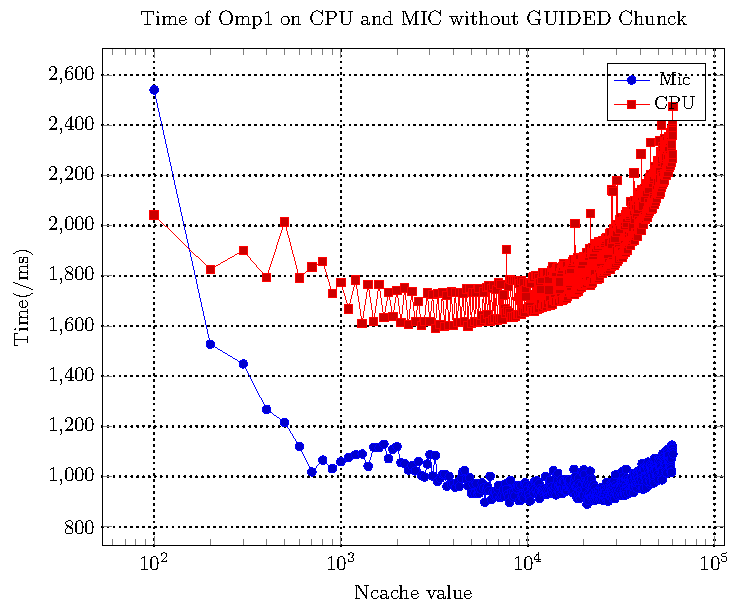
\includegraphics[width=\textwidth]{chap5/Figures/bsV1-6-mic-cpu-Time-Chunck-0.pdf}
   \caption{算法Omp1在不同Ncache值下的运行时间, $N=10^6$, $M=10$, 图中Omp1的运行时间随着Ncache的值先降低后增加,表明Ncache有一个
   最佳的取值范围。图中也可以看出同样地参数下算法在Xeon Phi平台上表现得比CPU平台下更好。由于M的取值较小,曲线具有一定的波动性。}
   \label{fig:v1-Ncache}
\end{figure}

我们发现算法在Xeon Phi上的表现优于CPU上的表现,并且当$10^4 < Ncache < 10^5$时,算法\ref{alg:omp1}在CPU和Xeon Phi上都存在一个最优化时间的窗口, 
这分别对应了CPU和Xeon Phi上的缓存大小,只有当
每次任务所需内存接近这个缓存大小时才能充分发挥性能。当我们考察Chunk值对算法的影响时,我们从图
\ref{fig:v1-mic-chunck-Ncache} \ref{fig:v1-cpu-chunck-Ncache} 中可以看到,取不同的Chunk值,
对算法的性能并没有明显的影响。
\begin{figure}[!t]
   \centering
   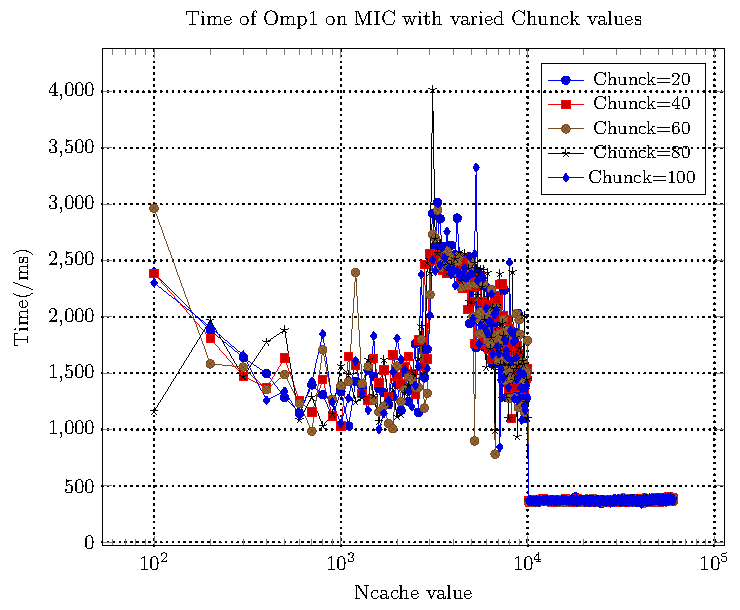
\includegraphics[width=\textwidth]{chap5/Figures/bsV1-mic-Time-Chunck.pdf}
   \caption{算法Omp1在MIC以及不同Chunk值下的时间, $N=10^5$, $M=10$, 图中当Ncache小于$10^4$时,各种Chunk值对应的曲线都有随机波动,但是
   并没有明显的优劣之分,而当$Ncache > 10^4$时,不同Chunk值的曲线都收敛在一起。}
   \label{fig:v1-mic-chunck-Ncache}
\end{figure}
这可以理解为,当一块Xeon Phi或者CPU上面的所有线程同时工作于一块Ncache大小的缓存区域时,每次分配给单个线程的任务量并不影响总的运算时间。
\begin{figure}[!t]
   \centering
   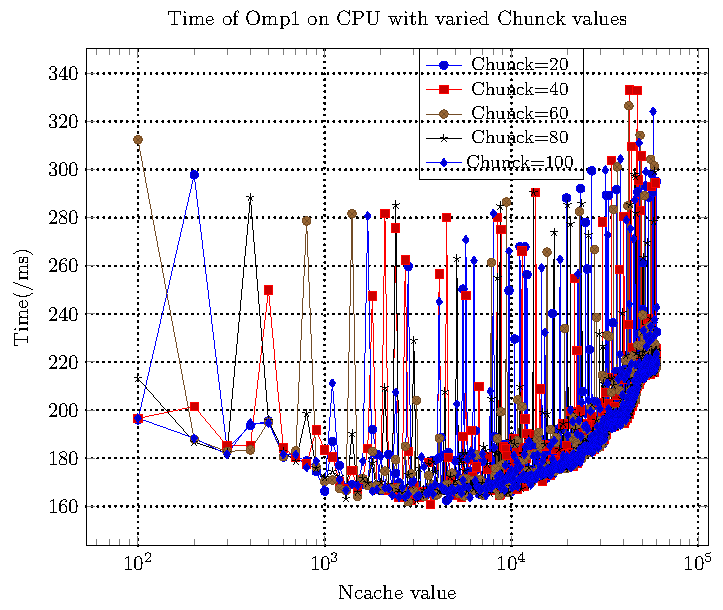
\includegraphics[width=\textwidth]{chap5/Figures/bsV1-CPU-Time-Chunck.pdf}
   \caption{算法Omp1在CPU以及不同Chunk值下运行时间对比, $N=10^5$, $M=10$, 图中的曲线出现较大的波动性,不同的Chunk值对应的曲线之间
   也没有明显的优劣,但所有的曲线都有一个明显的总体趋势,即有一个Ncache的最佳取值范围获得最好的性能}
   \label{fig:v1-cpu-chunck-Ncache}
\end{figure}
据此,我们可以直接利用系统自己智能非配的线程任务策略,而不同自己人为设定Chunk的大小。
\subsection{单机并行方案二的实验} % (fold)
\label{sub:bsV2}
在第二种单机并行方案中同样有两个重要的可调节参数,Nvec和Chunk值的大小(见算法\ref{alg:omp2_1}和\ref{alg:omp2_2})
同样的,我们先使用系统自己的线程任务分配机制(不设置Chunk值)。图\label{fig:v2-Nvec}中显示
算法在Xeon Phi上的性能优于CPU上的性能,并且当Nvec取值在500左右时可以使Xeon Phi发挥出最好的性能。
\begin{figure}[!t]
   \centering
   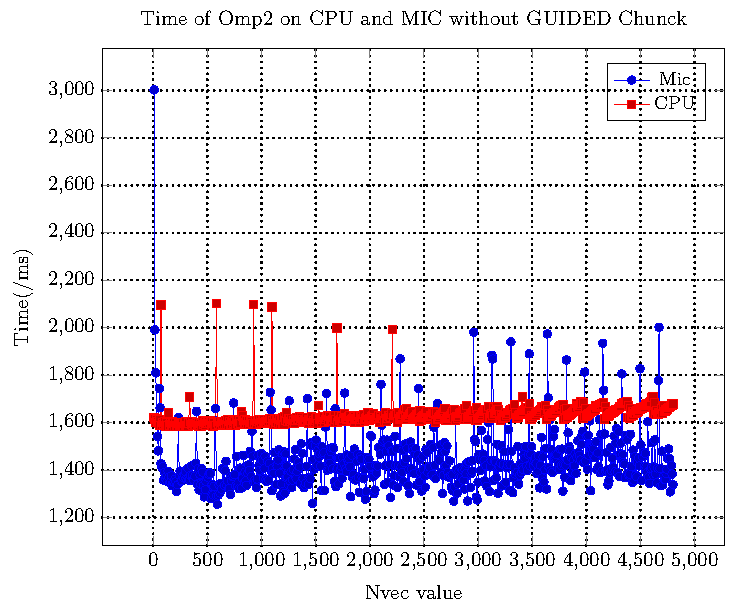
\includegraphics[width=\textwidth]{chap5/Figures/bsV2-6-mic-cpu-Time-Chunck-0.pdf}
   \caption{算法Omp2在不同Nvec值下的运行时间, $N=10^6$, $M=10$, CPU所代表的红色曲线波动性较小,随着Nvec的值也无明显变化,说明系统在默认的
   Chunk策略下自动进行了调整;同样Xeon Phi所代表的蓝色曲线虽然比红色曲线波动更大,但是总体趋势也是稳定在一个较优的性能上。}
   \label{fig:v2-Nvec}
\end{figure}
图\ref{fig:v2-mic-chunck-Nvec},\ref{fig:v2-cpu-chunck-Nvec}则反映出了取不同的Chunk值对性能的影响。当Nvec的值大于$10^3$后,计算速度
迅速下降,因为分配给单个核的内存任务超过了核本身的缓存大小,在这种情况下,取较小的Chunk的值可以获得相对理想的性能,因为这样单个核分配到的任务较小,
缓存对速度的影响较小。
\begin{figure}[!t]
   \centering
   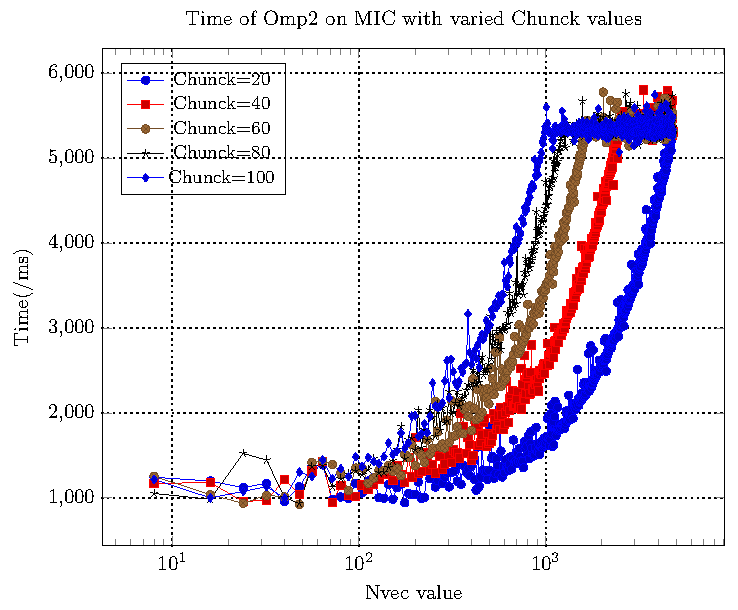
\includegraphics[width=\textwidth]{chap5/Figures/bsV2-mic-Time-Chunck.pdf}
   \caption{算法Omp2在MIC以及不同Chunk值下的时间, $N=10^5$, $M=10$, 可以明显地看到不同的曲线在Nvec的值大于100后出现了分离,较小值的Chunk策略
   获得了更好地性能,这是由于较小的单个线程任务量减弱了Nvec值超出单个核缓存造成的性能降低;而当Nvec的取值较小时不同的Chunk取值无明显区别。}
   \label{fig:v2-mic-chunck-Nvec}
\end{figure}
而当Nvec的值较小时,每个线程都能充分利用核上的缓存从而获得好的计算速度,而这时Chunk对性能的影响就很小了,我们在以后的实验中采用系统默认的Chunk方案,
或者Chunk为1的方案。
\begin{figure}[!t]
   \centering
   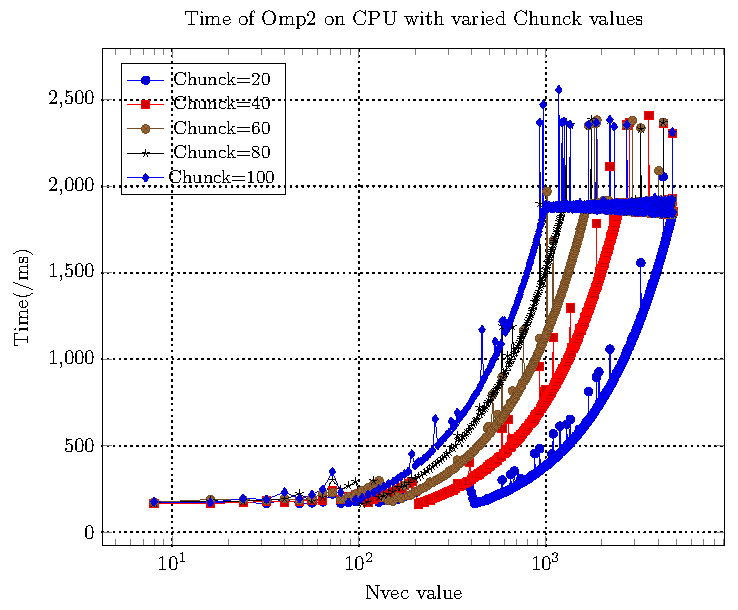
\includegraphics[width=\textwidth]{chap5/Figures/bsV2-CPU-Time-Chunck.pdf}
   \caption{算法Omp2在CPU以及不同Chunk值下运行时间对比, $N=10^5$, $M=10$}
   \label{fig:v2-cpu-chunck-Nvec}
\end{figure}

\subsection{两种单机并行方案的对比} % (fold)
\label{sub:compareV1V2}

在测试了我们的两种单机并行方案后,我们发现Xeon Phi能更好地发挥我们算法的性能。所以在对比两种算法优劣时,我们选择在Xeon Phi平台上进行测试。
图\label{fig:compareV1V2}对比了两种方案在Xeon Phi平台上不同OpenMP线程数下相对串行算法的加速比。
\begin{figure}[!t]
   \centering
   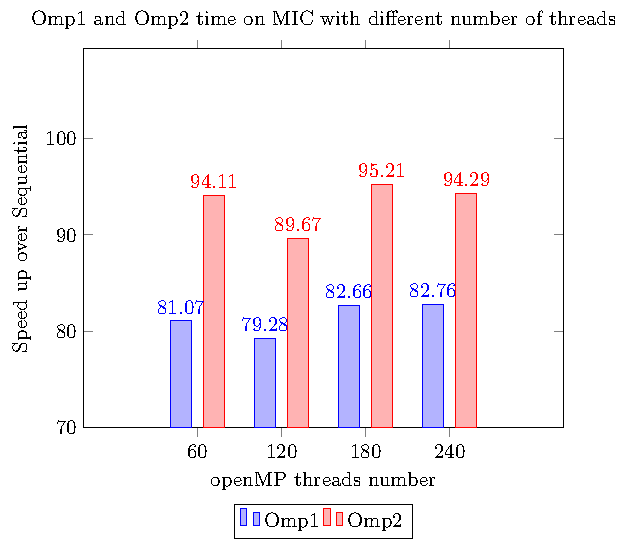
\includegraphics[width=\textwidth]{chap5/Figures/BS-Core-bar.pdf}
   \caption{Omp1, Omp2相对串行算法在MIC上的加速对比, Chunk 采用系统默认模式, $N=251988$, $M=100$, $Ncache=2000$, $Nvec=376$}
   \label{fig:compareV1V2}
\end{figure}
我们看到算法\ref{alg:omp2_1}和\ref{alg:omp2_2}明显优于算法\ref{alg:omp1}。算法\ref{alg:omp2_1}和\ref{alg:omp2_2}最大的加速比达到来了95倍。同时算法\ref{alg:omp1}在Xeon Phi 平台上也获得了
不错的加速比(80x)。考察单块Xeon Phi上的线程数对性能的影响,我们发现我们的算法在采用不同线程数(单核1线程,2线程,3线程和4线程)时性能的差别不是
很显著。主要原因是我们调优了两种算法的参数Ncache 和 Nvec。对于算法\ref{alg:omp1}来说,因为所有的数据都存储在Xeon Phi的缓存区,所以线程总数的改变
不会显著影响性能;对于算法\ref{alg:omp2_1}和\ref{alg:omp2_2}, 通过前面的分析,我们采用一个较小的Nvec值,可以使单个线程的任务装进单个核的缓存中,即使线程数量增加,也能
较好地发挥缓存的作用。

\section{多块Xeon Phi的并行结果分析} % (fold)
\label{sec:multiMIC}
在之前的分析基础上,我们认为算法\ref{alg:omp2_1}和\ref{alg:omp2_2}的表现优于算法\ref{alg:omp1}, 同时Xeon Phi平台的表现优于CPU平台。在这一小节中我们就要测试和分析
算法\ref{alg:omp2_1}和\ref{alg:omp2_2}在多个Xeon Phi环境下的严格扩展性(Strong Scalability)。受限制与实验设备,我们的Xeon Phi测试平台只有6块Xeon Phi处理器,并且
Xeon Phi处理器之间的连接速度并不理想。根据Pingpang测试的结果,我们发现两块Xeon Phi之间的通信速度只有307Mbyte/s,
但是由图\ref{fig:scale}中可知,我们的算法获得了超线性(superlinear)的扩展性。
\begin{figure}[!t]
   \centering
   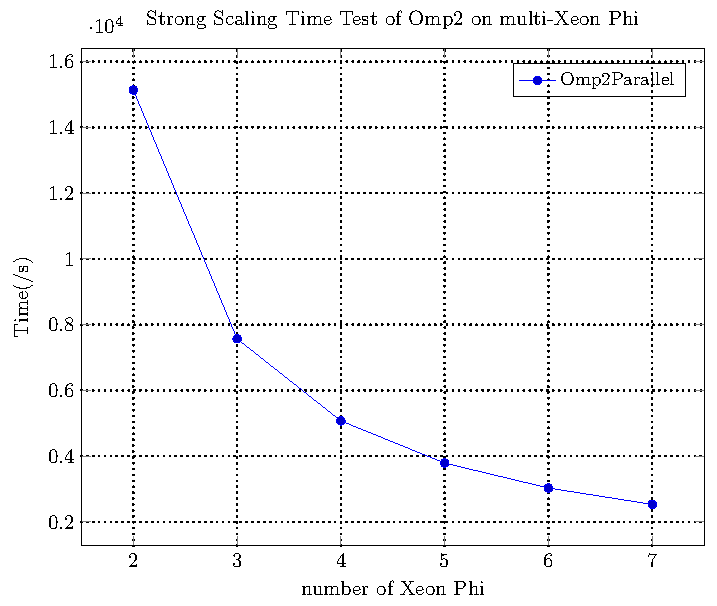
\includegraphics[width=\textwidth]{chap5/Figures/bsmpi-mic-scale.pdf}
   \caption{Omp2Parallel在multi-Xeon Phi上运行时间的严格扩展性$N=251988$, $M=10000$, $Ncache=2000$, $Nvec=192$。图中显示我们的算法
	   获得了超线性的扩展性能,这种超线性扩展的结果部分是由于我们的算法所基于的蒙特卡洛模拟。首先蒙特卡洛模拟需要大量的计算量来达到收敛性,
		   是个计算密集型的算法,其次蒙特卡洛各次模拟之间具有相互独立性,给算法上的实现提供了很大的潜在并行性。
		   同时我们的并行算法让单块Xeon Phi只负责一次蒙特卡洛的循环,这样各个Xeon Phi之间由于蒙特卡洛的独立性从而只有极小部分的通信需求,
		   这就使算法获得了非常理想的扩展性。}
   \label{fig:scale}
\end{figure}
这种超线性扩展的结果部分是由于我们的算法所基于的蒙特卡洛模拟。首先蒙特卡洛模拟需要大量的计算量来达到收敛性,是个计算密集型的算法,其次蒙特卡洛
各次模拟之间具有相互独立性,给算法上的实现提供了很大的潜在并行性。同时我们的并行算法让单块Xeon Phi只负责一次蒙特卡洛的循环,这样各个Xeon Phi之间
由于蒙特卡洛的独立性从而只有极小部分的通信需求, 这就使算法获得了非常理想的扩展性。

\section{算法的收敛性研究} % (fold)
\label{sec:converge}
我们模型和算法的最外层是通过二分法来搜索最小的符合条件的$N$值。通过增加蒙特卡洛模拟的次数$M$, 我们可以使搜索到得$N$值逐渐收敛到一个准确地值。
收敛性的测试是在一个有92个节点,184块Xeon E5的集群上进行测试。因为我们目前可供使用的Xeon Phi数量有限(6块),而收敛性测试所需要的$M$值
很大($10^6$), 我们才选择在CPU集群上进行测试。另一方面,我们的收敛性测试验证的是我们的算法,和运行平台无关,这也是我们选择CPU集群的原因。
图\ref{fig:converge}中显示当我们的$M$次数超过$10^4$,我们搜索到得$N$值已经收敛。而且整个收敛过程中,我们算法的效果随着$M$值的增大也未表现出
很大的波动性。
\begin{figure}[!t]
   \centering
   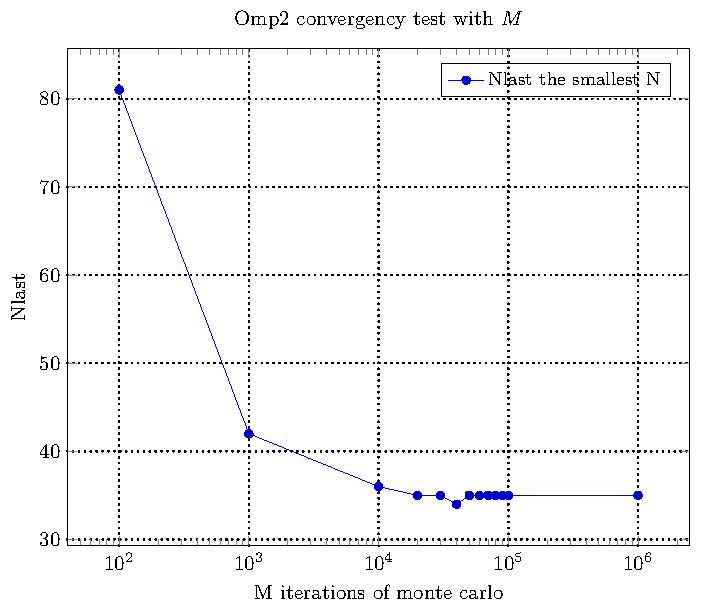
\includegraphics[width=\textwidth]{chap5/Figures/bs-converge.pdf}
   \caption{Omp2Parallel在multi-CPU上的收敛性, $N=251988$, $Nvec=192$ 当我们的$M$次数超过$10^4$,我们搜索到得$N$值已经收敛。
	   而且整个收敛过程中,我们算法的效果随着$M$值的增大也未表现出很大的波动性。}
   \label{fig:converge}
\end{figure}
这种良好的收敛性质使得我们的并行扩展性获得了意义,只要并行更多地处理器,就可以快速地收敛到我们所需要的$N$值。












\bibliographystyle{plain}
\bibliography{docear}

\end{document}


